% Options for packages loaded elsewhere
\PassOptionsToPackage{unicode}{hyperref}
\PassOptionsToPackage{hyphens}{url}
%
\documentclass[
]{article}
\usepackage{lmodern}
\usepackage{amssymb,amsmath}
\usepackage{ifxetex,ifluatex}
\ifnum 0\ifxetex 1\fi\ifluatex 1\fi=0 % if pdftex
  \usepackage[T1]{fontenc}
  \usepackage[utf8]{inputenc}
  \usepackage{textcomp} % provide euro and other symbols
\else % if luatex or xetex
  \usepackage{unicode-math}
  \defaultfontfeatures{Scale=MatchLowercase}
  \defaultfontfeatures[\rmfamily]{Ligatures=TeX,Scale=1}
\fi
% Use upquote if available, for straight quotes in verbatim environments
\IfFileExists{upquote.sty}{\usepackage{upquote}}{}
\IfFileExists{microtype.sty}{% use microtype if available
  \usepackage[]{microtype}
  \UseMicrotypeSet[protrusion]{basicmath} % disable protrusion for tt fonts
}{}
\makeatletter
\@ifundefined{KOMAClassName}{% if non-KOMA class
  \IfFileExists{parskip.sty}{%
    \usepackage{parskip}
  }{% else
    \setlength{\parindent}{0pt}
    \setlength{\parskip}{6pt plus 2pt minus 1pt}}
}{% if KOMA class
  \KOMAoptions{parskip=half}}
\makeatother
\usepackage{xcolor}
\IfFileExists{xurl.sty}{\usepackage{xurl}}{} % add URL line breaks if available
\IfFileExists{bookmark.sty}{\usepackage{bookmark}}{\usepackage{hyperref}}
\hypersetup{
  pdftitle={Do supporters help the home team win the match?},
  hidelinks,
  pdfcreator={LaTeX via pandoc}}
\urlstyle{same} % disable monospaced font for URLs
\usepackage[margin=1in]{geometry}
\usepackage{color}
\usepackage{fancyvrb}
\newcommand{\VerbBar}{|}
\newcommand{\VERB}{\Verb[commandchars=\\\{\}]}
\DefineVerbatimEnvironment{Highlighting}{Verbatim}{commandchars=\\\{\}}
% Add ',fontsize=\small' for more characters per line
\usepackage{framed}
\definecolor{shadecolor}{RGB}{248,248,248}
\newenvironment{Shaded}{\begin{snugshade}}{\end{snugshade}}
\newcommand{\AlertTok}[1]{\textcolor[rgb]{0.94,0.16,0.16}{#1}}
\newcommand{\AnnotationTok}[1]{\textcolor[rgb]{0.56,0.35,0.01}{\textbf{\textit{#1}}}}
\newcommand{\AttributeTok}[1]{\textcolor[rgb]{0.77,0.63,0.00}{#1}}
\newcommand{\BaseNTok}[1]{\textcolor[rgb]{0.00,0.00,0.81}{#1}}
\newcommand{\BuiltInTok}[1]{#1}
\newcommand{\CharTok}[1]{\textcolor[rgb]{0.31,0.60,0.02}{#1}}
\newcommand{\CommentTok}[1]{\textcolor[rgb]{0.56,0.35,0.01}{\textit{#1}}}
\newcommand{\CommentVarTok}[1]{\textcolor[rgb]{0.56,0.35,0.01}{\textbf{\textit{#1}}}}
\newcommand{\ConstantTok}[1]{\textcolor[rgb]{0.00,0.00,0.00}{#1}}
\newcommand{\ControlFlowTok}[1]{\textcolor[rgb]{0.13,0.29,0.53}{\textbf{#1}}}
\newcommand{\DataTypeTok}[1]{\textcolor[rgb]{0.13,0.29,0.53}{#1}}
\newcommand{\DecValTok}[1]{\textcolor[rgb]{0.00,0.00,0.81}{#1}}
\newcommand{\DocumentationTok}[1]{\textcolor[rgb]{0.56,0.35,0.01}{\textbf{\textit{#1}}}}
\newcommand{\ErrorTok}[1]{\textcolor[rgb]{0.64,0.00,0.00}{\textbf{#1}}}
\newcommand{\ExtensionTok}[1]{#1}
\newcommand{\FloatTok}[1]{\textcolor[rgb]{0.00,0.00,0.81}{#1}}
\newcommand{\FunctionTok}[1]{\textcolor[rgb]{0.00,0.00,0.00}{#1}}
\newcommand{\ImportTok}[1]{#1}
\newcommand{\InformationTok}[1]{\textcolor[rgb]{0.56,0.35,0.01}{\textbf{\textit{#1}}}}
\newcommand{\KeywordTok}[1]{\textcolor[rgb]{0.13,0.29,0.53}{\textbf{#1}}}
\newcommand{\NormalTok}[1]{#1}
\newcommand{\OperatorTok}[1]{\textcolor[rgb]{0.81,0.36,0.00}{\textbf{#1}}}
\newcommand{\OtherTok}[1]{\textcolor[rgb]{0.56,0.35,0.01}{#1}}
\newcommand{\PreprocessorTok}[1]{\textcolor[rgb]{0.56,0.35,0.01}{\textit{#1}}}
\newcommand{\RegionMarkerTok}[1]{#1}
\newcommand{\SpecialCharTok}[1]{\textcolor[rgb]{0.00,0.00,0.00}{#1}}
\newcommand{\SpecialStringTok}[1]{\textcolor[rgb]{0.31,0.60,0.02}{#1}}
\newcommand{\StringTok}[1]{\textcolor[rgb]{0.31,0.60,0.02}{#1}}
\newcommand{\VariableTok}[1]{\textcolor[rgb]{0.00,0.00,0.00}{#1}}
\newcommand{\VerbatimStringTok}[1]{\textcolor[rgb]{0.31,0.60,0.02}{#1}}
\newcommand{\WarningTok}[1]{\textcolor[rgb]{0.56,0.35,0.01}{\textbf{\textit{#1}}}}
\usepackage{graphicx,grffile}
\makeatletter
\def\maxwidth{\ifdim\Gin@nat@width>\linewidth\linewidth\else\Gin@nat@width\fi}
\def\maxheight{\ifdim\Gin@nat@height>\textheight\textheight\else\Gin@nat@height\fi}
\makeatother
% Scale images if necessary, so that they will not overflow the page
% margins by default, and it is still possible to overwrite the defaults
% using explicit options in \includegraphics[width, height, ...]{}
\setkeys{Gin}{width=\maxwidth,height=\maxheight,keepaspectratio}
% Set default figure placement to htbp
\makeatletter
\def\fps@figure{htbp}
\makeatother
\setlength{\emergencystretch}{3em} % prevent overfull lines
\providecommand{\tightlist}{%
  \setlength{\itemsep}{0pt}\setlength{\parskip}{0pt}}
\setcounter{secnumdepth}{-\maxdimen} % remove section numbering
\usepackage{booktabs}
\usepackage{longtable}
\usepackage{array}
\usepackage{multirow}
\usepackage{wrapfig}
\usepackage{float}
\usepackage{colortbl}
\usepackage{pdflscape}
\usepackage{tabu}
\usepackage{threeparttable}
\usepackage{threeparttablex}
\usepackage[normalem]{ulem}
\usepackage{makecell}
\usepackage{xcolor}

\title{Do supporters help the home team win the match?}
\author{CPES 2 - Example of research project

Detailed instructions in Lecture 16Grading system available hereLouis
Sirugue}
\date{Spring 2023}

\begin{document}
\maketitle

\hypertarget{i.-introduction}{%
\subsubsection{I. Introduction}\label{i.-introduction}}

It is well established that playing home at football grants an advantage
over the other team (Pollard, 1986). Yet, the specific determinants of
this advantage, and the extent of their respective contributions, has
not been clearly identified so far. The presence of local supporters in
the stadium ranks among the most plausible reasons for this stylized
fact, but whether or not supporters do help the team that plays home to
win a football match is a difficult question to answer given the small
variation in the presence of supporters at football matches. But by
preventing supporters to attend football matches, the COVID-19 pandemic
provides a unique setting to study this question. I study the effect of
the presence of supporters on the probability to win the match by
comparing the outcome of matches with supporters before the pandemic to
those without supporters after the pandemic.

Dowie (1982) was the first to elicit a home advantage at football. Even
though no causal effect could be identified, he stressed three potential
reasons: fatigue for the away team due to travel, familiarity with the
environment for the home team, and fans that support the home team and
may play on their motivation. Evidence for these three different
channels were then put forward in later studies. Concerning fatigue,
Pollard et al.~(2008) showed that distance traveled by the away team
significantly increases the number of expected goals in favor of the
home team by 0.115 goal per thousand kilometers traveled. Loughead et
al.~(2003) found mixed evidence about the familiarity hypothesis: high
quality teams suffered after a move from their familiar venue, whereas
low quality teams seemed to benefit from it. But overall, their results
provide little support for facility familiarity as an explanation for
the home advantage. Finally, Greer (1983) showed that booing from the
crowd at basketball games had a positive effect on performances of the
home team and negative effects for the team playing away. Still, the
overall effect of supporters on the outcome of sports events remains to
be quantified.

\hypertarget{ii.-data-cleaning}{%
\subsubsection{II. Data cleaning}\label{ii.-data-cleaning}}

I use data on every match of Premier League, Ligue 1, La Liga, and
Bundesliga from season 2018-2019 to season 2020-2021. The data is
publicly available at \href{https://fbref.com/}{fbref.com}, and
documents not only the score but also when and where the match took
place, as well as the number of supporters attending the match. Each of
the variables of the dataset is briefly described below.

\begin{Shaded}
\begin{Highlighting}[]
\CommentTok{# Load necessary packages}
\KeywordTok{library}\NormalTok{(tidyverse)  }\CommentTok{# To manipulate the data}
\KeywordTok{library}\NormalTok{(stargazer)  }\CommentTok{# To display regression results}
\KeywordTok{library}\NormalTok{(kableExtra) }\CommentTok{# To make html tables}

\CommentTok{# Import data from csv file}
\NormalTok{data_match <-}\StringTok{ }\KeywordTok{read.csv}\NormalTok{(}\StringTok{"data/data_match.csv"}\NormalTok{)}

\CommentTok{# Display the name of each variable}
\KeywordTok{names}\NormalTok{(data_match)}
\end{Highlighting}
\end{Shaded}

\begin{verbatim}
##  [1] "Wk"           "Day"          "Date"         "Time"         "Home"        
##  [6] "xG"           "Score"        "xG.1"         "Away"         "Attendance"  
## [11] "Venue"        "Referee"      "Match.Report" "Notes"        "League"      
## [16] "Season"
\end{verbatim}

The dataset contains 16 variables:

\begin{itemize}
\tightlist
\item
  \texttt{Wk}: Season week when the match took place\\
\item
  \texttt{Day}: Week day when the match took place\\
\item
  \texttt{Date}: Date of the match\\
\item
  \texttt{Time}: Time of the match\\
\item
  \texttt{Home}: Team that played home\\
\item
  \texttt{xG}: Expected number of goals for \emph{home} team\\
\item
  \texttt{Score}: Score of the match\\
\item
  \texttt{xG.1}: Expected number of goals for \emph{away} team\\
\item
  \texttt{Away}: Team that played away\\
\item
  \texttt{Attendance}: Number of supporters in the stadium
\item
  \texttt{Venue}: Name of the stadium where the match took place\\
\item
  \texttt{Referee}: Name of the referee\\
\item
  \texttt{Match.Report}: Link to an online report of the match\\
\item
  \texttt{Notes}: Miscellaneous information on the match\\
\item
  \texttt{League}: Name of the league\\
\item
  \texttt{Season}: Season from 2018-2019 to 2020-2021
\end{itemize}

Not all these variables are going to be useful, so I only keep the date
and time at which the match took place, the teams involved and the
score, the number of supporters in the stadium, the league and the
season. The following table displays the first five observations of the
data.

\begin{Shaded}
\begin{Highlighting}[]
\NormalTok{data_match <-}\StringTok{ }\NormalTok{data_match }\OperatorTok
\StringTok{  }\CommentTok{# Keep only the variables listed below in data_match}
\StringTok{  }\KeywordTok{select}\NormalTok{(Day, Date, Time, Home, Score, Away, Attendance, League, Season)}

\CommentTok{# Display the first five observations of the data}
\KeywordTok{kable}\NormalTok{(}\KeywordTok{head}\NormalTok{(data_match, }\DataTypeTok{n =} \DecValTok{5}\NormalTok{), }\DataTypeTok{caption =} \StringTok{"Outlook of the data:"}\NormalTok{)}
\end{Highlighting}
\end{Shaded}

\begin{table}

\caption{\label{tab:unnamed-chunk-2}Outlook of the data:}
\centering
\begin{tabular}[t]{llllllrll}
\toprule
Day & Date & Time & Home & Score & Away & Attendance & League & Season\\
\midrule
Fri & 2018-08-10 & 20:45 & Marseille & 4–0 & Toulouse & 60756 & Ligue 1 & 2018-2019\\
Sat & 2018-08-11 & 17:00 & Nantes & 1–3 & Monaco & 32760 & Ligue 1 & 2018-2019\\
Sat & 2018-08-11 & 20:00 & Montpellier & 1–2 & Dijon & 12765 & Ligue 1 & 2018-2019\\
Sat & 2018-08-11 & 20:00 & Lille & 3–1 & Rennes & 25708 & Ligue 1 & 2018-2019\\
Sat & 2018-08-11 & 20:00 & Angers & 3–4 & Nîmes & 9534 & Ligue 1 & 2018-2019\\
\bottomrule
\end{tabular}
\end{table}

Before starting the analysis, some variables must be recoded for
convenience. For instance, the \texttt{Score} variable is not in a
practical format. It stores the number of goals scored by each team,
separated with a dash. I should assign the score of each team to
distinct variables, and set their class to \texttt{numeric} instead of
\texttt{character}. The same type of modifications can be applied to the
\texttt{Time} variable, which in currently in \texttt{character} format
as \texttt{hh:mm}. To transform the time variable in a continuous
variable expressed in hours, the number of minutes divided by 60 should
be added to the number of hours. The following table displays the first
15 lines of the data recoded as described above.

\begin{Shaded}
\begin{Highlighting}[]
\NormalTok{data_match <-}\StringTok{ }\NormalTok{data_match }\OperatorTok
\StringTok{         }\CommentTok{# Assign the first and third characters of the string Score to Goals_home and Goals_away}
\StringTok{  }\KeywordTok{mutate}\NormalTok{(}\DataTypeTok{Goals_home =} \KeywordTok{as.numeric}\NormalTok{(}\KeywordTok{substr}\NormalTok{(Score, }\DecValTok{1}\NormalTok{, }\DecValTok{1}\NormalTok{)),}
         \DataTypeTok{Goals_away =} \KeywordTok{as.numeric}\NormalTok{(}\KeywordTok{substr}\NormalTok{(Score, }\DecValTok{3}\NormalTok{, }\DecValTok{3}\NormalTok{)),}
         \CommentTok{# Generate a variable for the outcome of the match depending on who scored the most}
         \DataTypeTok{Winner =} \KeywordTok{case_when}\NormalTok{(Goals_home }\OperatorTok{>}\StringTok{ }\NormalTok{Goals_away }\OperatorTok{~}\StringTok{ "Home"}\NormalTok{,}
\NormalTok{                            Goals_home }\OperatorTok{==}\StringTok{ }\NormalTok{Goals_away }\OperatorTok{~}\StringTok{ "Draw"}\NormalTok{,}
\NormalTok{                            Goals_home }\OperatorTok{<}\StringTok{ }\NormalTok{Goals_away }\OperatorTok{~}\StringTok{ "Away"}\NormalTok{),}
         \CommentTok{# Recode the Time variable as a continuous variable}
         \DataTypeTok{Time =} \KeywordTok{as.numeric}\NormalTok{(}\KeywordTok{substr}\NormalTok{(Time, }\DecValTok{1}\NormalTok{, }\DecValTok{2}\NormalTok{)) }\OperatorTok{+}\StringTok{ }\KeywordTok{as.numeric}\NormalTok{(}\KeywordTok{substr}\NormalTok{(Time, }\DecValTok{4}\NormalTok{, }\DecValTok{5}\NormalTok{)) }\OperatorTok{/}\StringTok{ }\DecValTok{60}\NormalTok{)}

\CommentTok{# Display the first 15 rows of the recoded data}
\KeywordTok{kable}\NormalTok{(}\KeywordTok{head}\NormalTok{(data_match, }\DataTypeTok{n =} \DecValTok{15}\NormalTok{), }\DataTypeTok{caption =} \StringTok{"Recoded data:"}\NormalTok{)}
\end{Highlighting}
\end{Shaded}

\begin{table}

\caption{\label{tab:unnamed-chunk-3}Recoded data:}
\centering
\begin{tabular}[t]{llrlllrllrrl}
\toprule
Day & Date & Time & Home & Score & Away & Attendance & League & Season & Goals\_home & Goals\_away & Winner\\
\midrule
Fri & 2018-08-10 & 20.75 & Marseille & 4–0 & Toulouse & 60756 & Ligue 1 & 2018-2019 & 4 & 0 & Home\\
Sat & 2018-08-11 & 17.00 & Nantes & 1–3 & Monaco & 32760 & Ligue 1 & 2018-2019 & 1 & 3 & Away\\
Sat & 2018-08-11 & 20.00 & Montpellier & 1–2 & Dijon & 12765 & Ligue 1 & 2018-2019 & 1 & 2 & Away\\
Sat & 2018-08-11 & 20.00 & Lille & 3–1 & Rennes & 25708 & Ligue 1 & 2018-2019 & 3 & 1 & Home\\
Sat & 2018-08-11 & 20.00 & Angers & 3–4 & Nîmes & 9534 & Ligue 1 & 2018-2019 & 3 & 4 & Away\\
\addlinespace
Sat & 2018-08-11 & 20.00 & Saint-Étienne & 2–1 & Guingamp & 26006 & Ligue 1 & 2018-2019 & 2 & 1 & Home\\
Sat & 2018-08-11 & 20.00 & Nice & 0–1 & Reims & 21421 & Ligue 1 & 2018-2019 & 0 & 1 & Away\\
Sun & 2018-08-12 & 15.00 & Lyon & 2–0 & Amiens & 48263 & Ligue 1 & 2018-2019 & 2 & 0 & Home\\
Sun & 2018-08-12 & 17.00 & Bordeaux & 0–2 & Strasbourg & 23079 & Ligue 1 & 2018-2019 & 0 & 2 & Away\\
Sun & 2018-08-12 & 21.00 & Paris S-G & 3–0 & Caen & 47289 & Ligue 1 & 2018-2019 & 3 & 0 & Home\\
\addlinespace
 &  & NA &  &  &  & NA & Ligue 1 & 2018-2019 & NA & NA & NA\\
Fri & 2018-08-17 & 20.75 & Reims & 1–0 & Lyon & 18917 & Ligue 1 & 2018-2019 & 1 & 0 & Home\\
Sat & 2018-08-18 & 17.00 & Guingamp & 1–3 & Paris S-G & 19003 & Ligue 1 & 2018-2019 & 1 & 3 & Away\\
Sat & 2018-08-18 & 20.00 & Amiens & 1–2 & Montpellier & 10402 & Ligue 1 & 2018-2019 & 1 & 2 & Away\\
Sat & 2018-08-18 & 20.00 & Rennes & 1–0 & Angers & 19300 & Ligue 1 & 2018-2019 & 1 & 0 & Home\\
\bottomrule
\end{tabular}
\end{table}

An important step of the data cleaning process is to handle missing
values. It can be seen from the table above that between each week of
competition there is an empty line with missing values. These rows can
be deleted by filtering out every observation for which the
\texttt{Score} variable is blank.

\begin{Shaded}
\begin{Highlighting}[]
\CommentTok{# Drop blank rows}
\NormalTok{data_match <-}\StringTok{ }\NormalTok{data_match }\OperatorTok\StringTok{ }\KeywordTok{filter}\NormalTok{(Score }\OperatorTok{!=}\StringTok{ ""}\NormalTok{)}
\end{Highlighting}
\end{Shaded}

To check for the presence of actual missing values in the data, the
following table shows the number of missing values for each variable of
the dataset.

\begin{Shaded}
\begin{Highlighting}[]
\CommentTok{# Show the number of missing values for each variable}
\KeywordTok{kable}\NormalTok{(data_match }\OperatorTok\StringTok{ }\KeywordTok{summarise_all}\NormalTok{(}\OperatorTok{~}\KeywordTok{sum}\NormalTok{(}\KeywordTok{is.na}\NormalTok{(.))), }
      \DataTypeTok{caption =} \StringTok{"Number of missing values per variable:"}\NormalTok{)}
\end{Highlighting}
\end{Shaded}

\begin{table}

\caption{\label{tab:unnamed-chunk-5}Number of missing values per variable:}
\centering
\begin{tabular}[t]{rrrrrrrrrrrr}
\toprule
Day & Date & Time & Home & Score & Away & Attendance & League & Season & Goals\_home & Goals\_away & Winner\\
\midrule
0 & 0 & 0 & 0 & 0 & 0 & 1670 & 0 & 0 & 0 & 0 & 0\\
\bottomrule
\end{tabular}
\end{table}

The only variable with missing values is \texttt{Attendance}. There are
1670 matches for which the number of supporters in the stadium is not
reported. To get a better understanding of what is going on with this
variable, the following table summarizes the distribution of
\texttt{Attendance} with its minimum and its maximum value, its mean,
and the three quartiles.

\begin{Shaded}
\begin{Highlighting}[]
\CommentTok{# Display the summary statistics of the Attendance variable}
\KeywordTok{kable}\NormalTok{(}\KeywordTok{as.matrix}\NormalTok{(}\KeywordTok{summary}\NormalTok{(data_match}\OperatorTok{$}\NormalTok{Attendance)) }\OperatorTok\StringTok{ }\KeywordTok{t}\NormalTok{(), }
      \DataTypeTok{caption =} \StringTok{"Attendance - Descriptive statistics:"}\NormalTok{)}
\end{Highlighting}
\end{Shaded}

\begin{table}

\caption{\label{tab:unnamed-chunk-6}Attendance - Descriptive statistics:}
\centering
\begin{tabular}[t]{rrrrrrr}
\toprule
Min. & 1st Qu. & Median & Mean & 3rd Qu. & Max. & NA's\\
\midrule
13 & 16158 & 27717 & 31789.99 & 45014 & 93426 & 1670\\
\bottomrule
\end{tabular}
\end{table}

The number of spectators per match ranges from 13 to 93426. But due to
the COVID-19 pandemic that prevented many matches from having supporters
in the stadium, there should be values of \texttt{Attendance} equal to
0. It is thus possible that the missing values of \texttt{Attendance}
are actually these matches where no supporter was allowed to attend the
event, and that missing values are actually not missing but a way of
coding no attendance. This hypothesis is even more plausible given that
other than the \texttt{Attendance} variable, there is no issue of
missing value in the data. A visual check can be conducted to test this
hypothesis, by recoding missing values to 0 and showing the monthly
evolution of the average number of supporters in stadiums. This can be
done separately for each league to see whether or not the issue is
league-specific.

\begin{Shaded}
\begin{Highlighting}[]
\NormalTok{attendance_data <-}\StringTok{ }\NormalTok{data_match }\OperatorTok
\StringTok{         }\CommentTok{# Replace missing values of Attendance by 0}
\StringTok{  }\KeywordTok{mutate}\NormalTok{(}\DataTypeTok{Attendance =} \KeywordTok{ifelse}\NormalTok{(}\KeywordTok{is.na}\NormalTok{(Attendance), }\DecValTok{0}\NormalTok{, Attendance),}
         \CommentTok{# Keep only the YYYY-MM part of the Date variable (YYYY-MM-DD)}
         \DataTypeTok{Month =} \KeywordTok{substr}\NormalTok{(Date, }\DecValTok{1}\NormalTok{, }\DecValTok{7}\NormalTok{)) }\OperatorTok
\StringTok{  }\CommentTok{# Do computations separately for each month and each league}
\StringTok{  }\KeywordTok{group_by}\NormalTok{(Month, League) }\OperatorTok
\StringTok{  }\CommentTok{# Compute the average number of supporters in the stadium}
\StringTok{  }\KeywordTok{summarize}\NormalTok{(}\DataTypeTok{Attendance =} \KeywordTok{mean}\NormalTok{(Attendance)) }\OperatorTok
\StringTok{  }\CommentTok{# Sort the data by ascending order of month and group by month}
\StringTok{  }\KeywordTok{ungroup}\NormalTok{() }\OperatorTok\StringTok{ }\KeywordTok{arrange}\NormalTok{(Month) }\OperatorTok\StringTok{  }\KeywordTok{group_by}\NormalTok{(Month) }\OperatorTok
\StringTok{  }\CommentTok{# Attribute a number from 1 to N to each month whatever the league}
\StringTok{  }\KeywordTok{mutate}\NormalTok{(}\DataTypeTok{Month_id =} \KeywordTok{cur_group_id}\NormalTok{())}

\KeywordTok{ggplot}\NormalTok{(attendance_data, }
       \CommentTok{# Assign month/attendance to the x-/y-axis and one color per league}
       \KeywordTok{aes}\NormalTok{(}\DataTypeTok{x =}\NormalTok{ Month_id, }\DataTypeTok{y =}\NormalTok{ Attendance, }\DataTypeTok{color =}\NormalTok{ League), }\DataTypeTok{alpha =} \FloatTok{.75}\NormalTok{) }\OperatorTok{+}
\StringTok{  }\CommentTok{# Draw a line and a point geometry and rename legend}
\StringTok{  }\KeywordTok{geom_line}\NormalTok{(}\DataTypeTok{size =} \FloatTok{1.2}\NormalTok{) }\OperatorTok{+}\StringTok{ }\KeywordTok{geom_point}\NormalTok{(}\DataTypeTok{size =} \FloatTok{1.5}\NormalTok{) }\OperatorTok{+}\StringTok{ }\KeywordTok{labs}\NormalTok{(}\DataTypeTok{color =} \StringTok{"League:"}\NormalTok{) }\OperatorTok{+}
\StringTok{  }\CommentTok{# Label the x axis with months in character format}
\StringTok{  }\KeywordTok{scale_x_continuous}\NormalTok{(}\DataTypeTok{name =} \StringTok{"Month"}\NormalTok{, }\DataTypeTok{breaks =} \KeywordTok{unique}\NormalTok{(attendance_data}\OperatorTok{$}\NormalTok{Month_id), }
                     \DataTypeTok{labels =} \KeywordTok{unique}\NormalTok{(attendance_data}\OperatorTok{$}\NormalTok{Month)) }\OperatorTok{+}\StringTok{ }
\StringTok{  }\CommentTok{# Rotate the month labels by 90 degrees}
\StringTok{  }\KeywordTok{theme}\NormalTok{(}\DataTypeTok{axis.text.x =} \KeywordTok{element_text}\NormalTok{(}\DataTypeTok{angle =} \DecValTok{90}\NormalTok{, }\DataTypeTok{vjust =} \FloatTok{0.5}\NormalTok{, }\DataTypeTok{hjust =} \DecValTok{1}\NormalTok{))}
\end{Highlighting}
\end{Shaded}

\begin{center}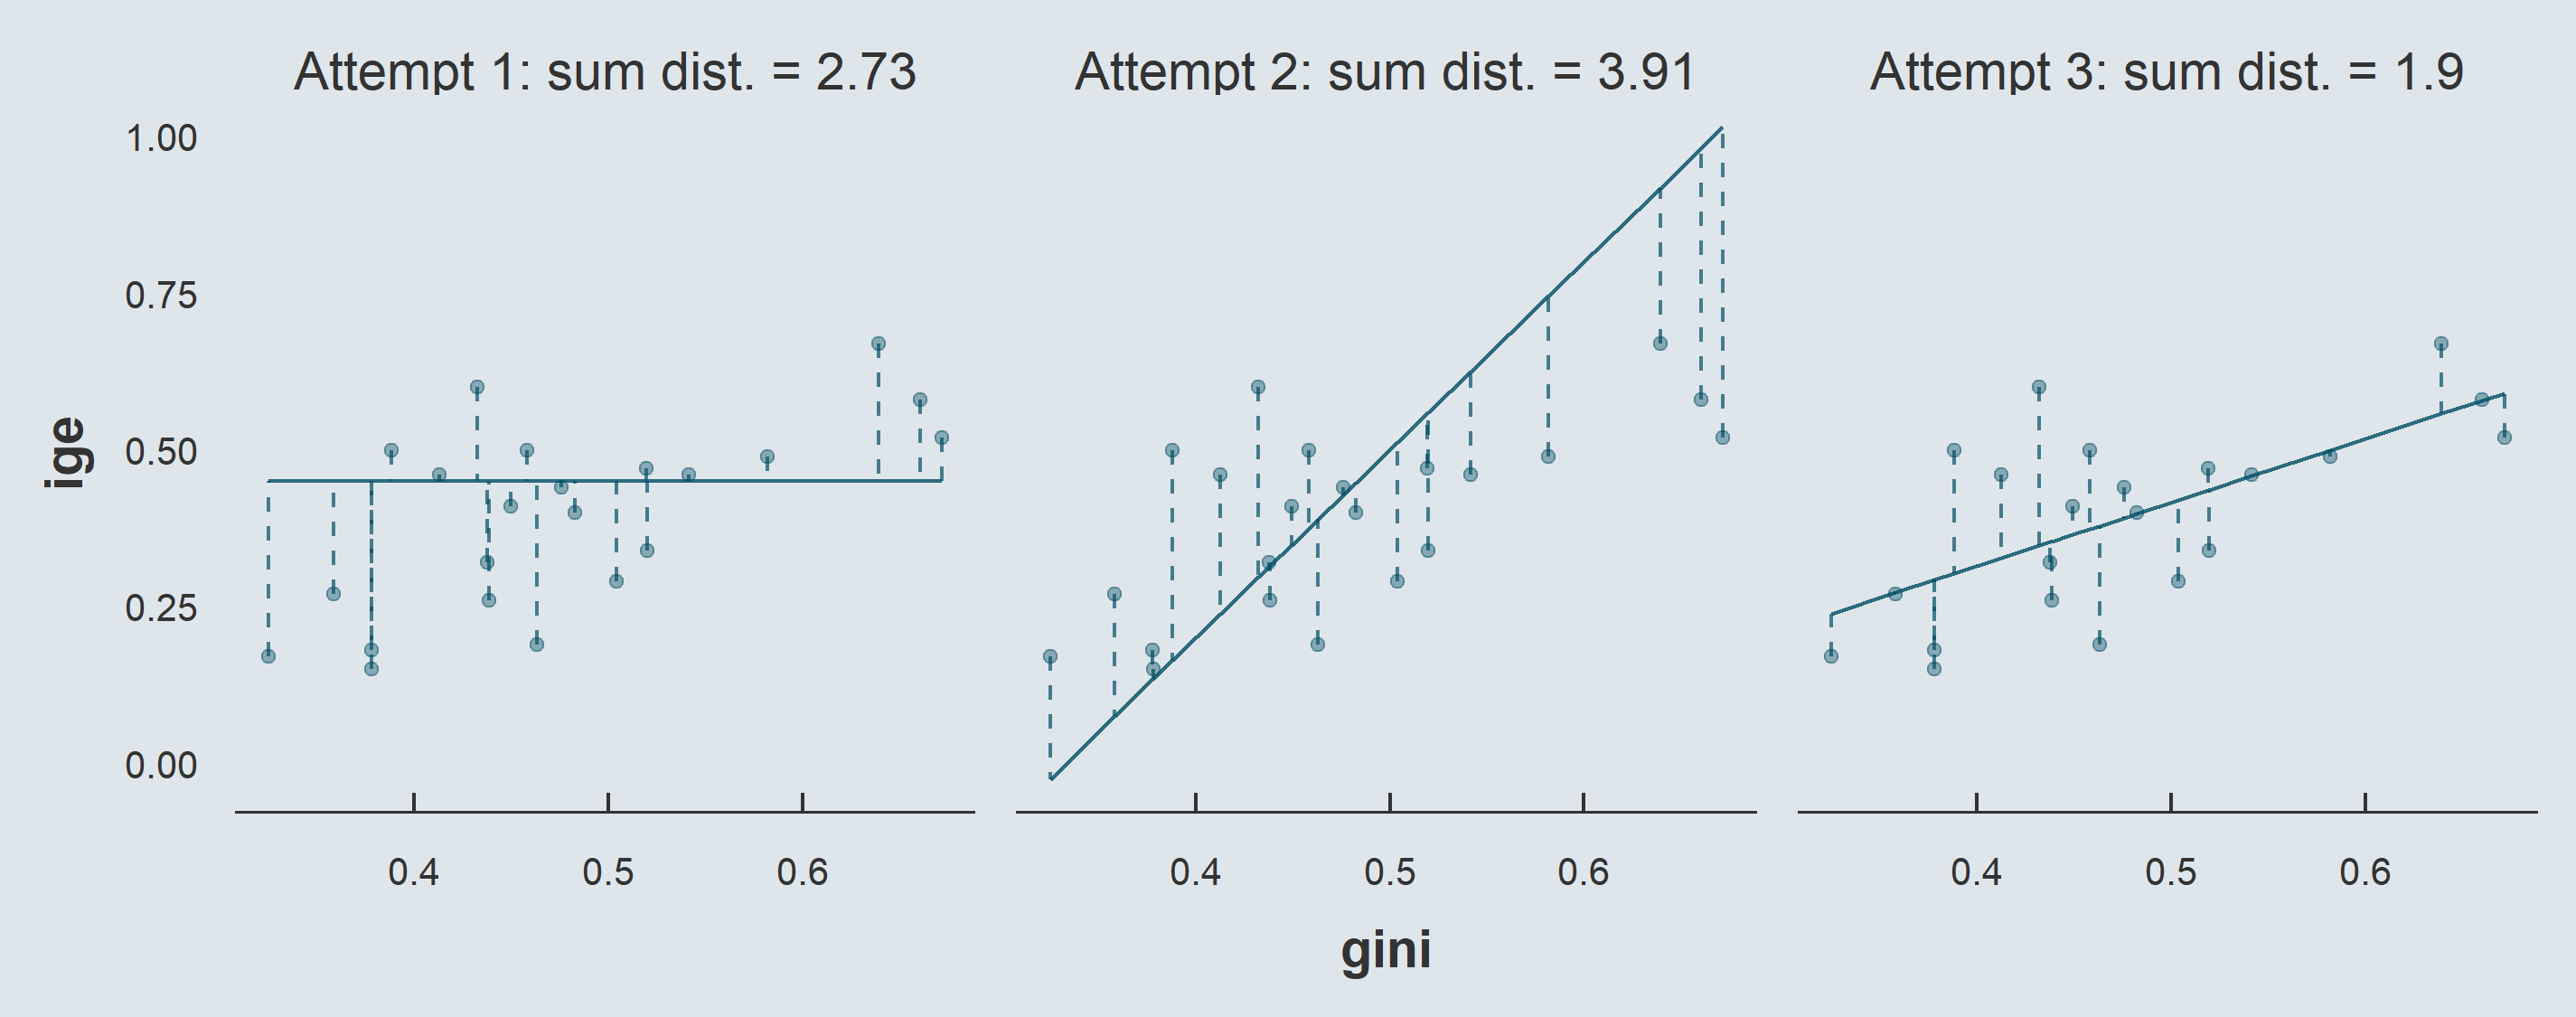
\includegraphics{example_files/figure-latex/unnamed-chunk-7-1} \end{center}

The sudden drop to 0 attendance due to the pandemic right after March
2020 is striking, and confirms that the missing values of the
\texttt{Attendance} variable should indeed be recoded as 0. It also
illustrates that the COVID-19 pandemic provides an ideal setting to test
for the potential effect of the presence of supporters in the stadium on
the probability for the home team to win the match.

\begin{Shaded}
\begin{Highlighting}[]
\CommentTok{# Replace missing values of Attendance by 0}
\NormalTok{data_match <-}\StringTok{ }\NormalTok{data_match }\OperatorTok\StringTok{ }\KeywordTok{mutate}\NormalTok{(}\DataTypeTok{Attendance =} \KeywordTok{ifelse}\NormalTok{(}\KeywordTok{is.na}\NormalTok{(Attendance), }\DecValTok{0}\NormalTok{, Attendance))}
\end{Highlighting}
\end{Shaded}

\hypertarget{iii.-descriptive-statistics}{%
\subsubsection{III. Descriptive
statistics}\label{iii.-descriptive-statistics}}

Once the data is cleaned and recoded, it should be described with
appropriate statistics. The first relevant information is the number of
observations. The observation level of the data being the match, the
following table displays the number of matches in the data separately
for each league and each season.

\begin{Shaded}
\begin{Highlighting}[]
\NormalTok{nb_obs <-}\StringTok{ }\NormalTok{data_match }\OperatorTok
\StringTok{  }\CommentTok{# Do computations separately for each season and each league}
\StringTok{  }\KeywordTok{group_by}\NormalTok{(League, Season) }\OperatorTok
\StringTok{  }\CommentTok{# Compute the number of match per season/league}
\StringTok{  }\KeywordTok{summarise}\NormalTok{(}\DataTypeTok{n_match =} \KeywordTok{n}\NormalTok{()) }\OperatorTok\StringTok{ }
\StringTok{  }\CommentTok{# Put these values in separate columns for each season}
\StringTok{  }\KeywordTok{pivot_wider}\NormalTok{(}\DataTypeTok{names_from =} \StringTok{"Season"}\NormalTok{, }\DataTypeTok{values_from =} \StringTok{"n_match"}\NormalTok{) }\OperatorTok
\StringTok{  }\CommentTok{# Compute the total number of matches per league}
\StringTok{  }\KeywordTok{mutate}\NormalTok{(}\DataTypeTok{Total =} \StringTok{`}\DataTypeTok{2018-2019}\StringTok{`} \OperatorTok{+}\StringTok{ `}\DataTypeTok{2019-2020}\StringTok{`} \OperatorTok{+}\StringTok{ `}\DataTypeTok{2020-2021}\StringTok{`}\NormalTok{) }

\NormalTok{nb_obs }\OperatorTok
\StringTok{  }\CommentTok{# Add one Total row which is the sum of all the above}
\StringTok{  }\KeywordTok{bind_rows}\NormalTok{(nb_obs }\OperatorTok\StringTok{ }\KeywordTok{mutate}\NormalTok{(}\DataTypeTok{League =} \StringTok{"Total"}\NormalTok{) }\OperatorTok\StringTok{ }\KeywordTok{group_by}\NormalTok{(League) }\OperatorTok\StringTok{ }\KeywordTok{summarise_all}\NormalTok{(}\OperatorTok{~}\KeywordTok{sum}\NormalTok{(.))) }\OperatorTok
\StringTok{  }\CommentTok{# Display in an htlm table}
\StringTok{  }\KeywordTok{kable}\NormalTok{(.,  }\DataTypeTok{caption =} \StringTok{"Number of matches:"}\NormalTok{) }\OperatorTok
\StringTok{  }\CommentTok{# Set characters in the column Total in bold}
\StringTok{  }\KeywordTok{column_spec}\NormalTok{(}\DecValTok{5}\NormalTok{, }\DataTypeTok{bold =}\NormalTok{ T) }\OperatorTok
\StringTok{  }\CommentTok{# Set characters in the row Total in bold}
\StringTok{  }\KeywordTok{row_spec}\NormalTok{(}\DecValTok{5}\NormalTok{, }\DataTypeTok{bold =}\NormalTok{ T) }
\end{Highlighting}
\end{Shaded}

\begin{table}

\caption{\label{tab:unnamed-chunk-9}Number of matches:}
\centering
\begin{tabular}[t]{lrrr>{}r}
\toprule
League & 2018-2019 & 2019-2020 & 2020-2021 & Total\\
\midrule
Bundesliga & 306 & 306 & 306 & \textbf{918}\\
La Liga & 380 & 380 & 380 & \textbf{1140}\\
Ligue 1 & 380 & 279 & 380 & \textbf{1039}\\
Premier League & 380 & 380 & 380 & \textbf{1140}\\
\textbf{Total} & \textbf{1446} & \textbf{1345} & \textbf{1446} & \textbf{\textbf{4237}}\\
\bottomrule
\end{tabular}
\end{table}

The data contains a total number of 4237 observations, with slightly
less observations in the 2019-2020 season than in the two others due to
the cancellation of matches in Ligue 1. Besides this event, each league
has 380 matches per season except the Bundesliga for which the number of
matches per season amounts to 306. The following table shows the number
of matches won home, away, and the number of draws, along with their
respective proportion in the dataset.

\begin{Shaded}
\begin{Highlighting}[]
\NormalTok{data_match }\OperatorTok
\StringTok{  }\CommentTok{# Do computations separately for each outcome}
\StringTok{  }\KeywordTok{group_by}\NormalTok{(Winner) }\OperatorTok
\StringTok{  }\CommentTok{# Compute the number of observations and the percentage}
\StringTok{  }\KeywordTok{summarise}\NormalTok{(}\DataTypeTok{N =} \KeywordTok{n}\NormalTok{(), }\DataTypeTok{Pct =} \KeywordTok{n}\NormalTok{() }\OperatorTok{/}\StringTok{ }\KeywordTok{nrow}\NormalTok{(.)) }\OperatorTok
\StringTok{  }\CommentTok{# Display in an html table}
\StringTok{  }\KeywordTok{kable}\NormalTok{(., }\StringTok{"Distribution of match outcomes"}\NormalTok{)}
\end{Highlighting}
\end{Shaded}

\begin{table}

\caption{\label{tab:unnamed-chunk-10}Distribution of match outcomes}
\centering
\begin{tabular}[t]{lrr}
\toprule
Winner & N & Pct\\
\midrule
Away & 1343 & 0.32\\
Draw & 1067 & 0.25\\
Home & 1827 & 0.43\\
\bottomrule
\end{tabular}
\end{table}

This confirm the well-established stylized fact that football matches
have greater chance to be won by the home team. To provide an overview
of the variables that are used in this analysis, the following tables
summarizes the distribution of the three main variables: the number of
supporters in the stadium, the number of goals scored by the team that
plays home, and that scored by the team that plays away. These
statistics are provided separately for each league and each season.

\begin{Shaded}
\begin{Highlighting}[]
\NormalTok{descriptive_data <-}\StringTok{ }\NormalTok{data_match }\OperatorTok
\StringTok{  }\CommentTok{# Put the variables of interest in long format}
\StringTok{  }\KeywordTok{pivot_longer}\NormalTok{(}\KeywordTok{c}\NormalTok{(Attendance, Goals_home, Goals_away), }
               \DataTypeTok{names_to =} \StringTok{"Variable"}\NormalTok{, }\DataTypeTok{values_to =} \StringTok{"Value"}\NormalTok{) }\OperatorTok
\StringTok{  }\CommentTok{# Group the data by variable of interest, season, and league}
\StringTok{  }\KeywordTok{group_by}\NormalTok{(Variable, Season, League) }\OperatorTok
\StringTok{  }\CommentTok{# Compute the descriptive statistics}
\StringTok{  }\KeywordTok{summarise}\NormalTok{(}\DataTypeTok{Min =} \KeywordTok{min}\NormalTok{(Value), }
            \DataTypeTok{Q1 =} \KeywordTok{quantile}\NormalTok{(Value, }\DecValTok{1}\OperatorTok{/}\DecValTok{4}\NormalTok{),}
            \DataTypeTok{Median =} \KeywordTok{median}\NormalTok{(Value), }
            \DataTypeTok{Mean =} \KeywordTok{mean}\NormalTok{(Value), }
            \DataTypeTok{Q3 =} \KeywordTok{quantile}\NormalTok{(Value, }\DecValTok{3}\OperatorTok{/}\DecValTok{4}\NormalTok{),}
            \DataTypeTok{Max =} \KeywordTok{max}\NormalTok{(Value)) }\OperatorTok
\StringTok{  }\CommentTok{# Ungroup the data}
\StringTok{  }\KeywordTok{ungroup}\NormalTok{()}
\end{Highlighting}
\end{Shaded}

\hypertarget{section}{%
\paragraph{}\label{section}}

\hypertarget{section-1}{%
\subparagraph{2018-2019}\label{section-1}}

\begin{Shaded}
\begin{Highlighting}[]
\NormalTok{descriptive_data }\OperatorTok\StringTok{ }
\StringTok{  }\CommentTok{# Keep only the observations of the 2018-2019 season}
\StringTok{  }\KeywordTok{filter}\NormalTok{(Season }\OperatorTok{==}\StringTok{ "2018-2019"}\NormalTok{) }\OperatorTok\StringTok{ }
\StringTok{  }\CommentTok{# Keep only the variables to display}
\StringTok{  }\KeywordTok{select}\NormalTok{(}\OperatorTok{-}\KeywordTok{c}\NormalTok{(Variable, Season)) }\OperatorTok
\StringTok{  }\CommentTok{# Add a caption to the table}
\StringTok{  }\KeywordTok{kable}\NormalTok{(., }\DataTypeTok{caption =} \KeywordTok{paste}\NormalTok{(}\StringTok{"Season"}\NormalTok{, }\StringTok{"2018-2019"}\NormalTok{)) }\OperatorTok
\StringTok{  }\CommentTok{# Display the name of the variable for the corresponding rows}
\StringTok{  }\KeywordTok{pack_rows}\NormalTok{(}\StringTok{"Attendance"}\NormalTok{, }\DecValTok{1}\NormalTok{, }\DecValTok{4}\NormalTok{) }\OperatorTok
\StringTok{  }\KeywordTok{pack_rows}\NormalTok{(}\StringTok{"Goals away"}\NormalTok{, }\DecValTok{5}\NormalTok{, }\DecValTok{8}\NormalTok{) }\OperatorTok
\StringTok{  }\KeywordTok{pack_rows}\NormalTok{(}\StringTok{"Goals home"}\NormalTok{, }\DecValTok{9}\NormalTok{, }\DecValTok{12}\NormalTok{)}
\end{Highlighting}
\end{Shaded}

\begin{table}

\caption{\label{tab:unnamed-chunk-12}Season 2018-2019}
\centering
\begin{tabular}[t]{lrrrrrr}
\toprule
League & Min & Q1 & Median & Mean & Q3 & Max\\
\midrule
\addlinespace[0.3em]
\multicolumn{7}{l}{\textbf{Attendance}}\\
\hspace{1em}Bundesliga & 19205 & 29230.50 & 40911.0 & 43453.18 & 52500.00 & 81365\\
\hspace{1em}La Liga & 3592 & 12074.50 & 19367.5 & 27118.68 & 39587.75 & 93265\\
\hspace{1em}Ligue 1 & 0 & 12795.75 & 17577.5 & 22807.27 & 27378.50 & 64696\\
\hspace{1em}Premier League & 9980 & 25034.75 & 31948.0 & 38181.29 & 53282.75 & 81332\\
\addlinespace[0.3em]
\multicolumn{7}{l}{\textbf{Goals away}}\\
\hspace{1em}Bundesliga & 0 & 0.00 & 1.0 & 1.39 & 2.00 & 6\\
\hspace{1em}La Liga & 0 & 0.00 & 1.0 & 1.13 & 2.00 & 6\\
\hspace{1em}Ligue 1 & 0 & 0.00 & 1.0 & 1.09 & 2.00 & 5\\
\hspace{1em}Premier League & 0 & 0.00 & 1.0 & 1.25 & 2.00 & 6\\
\addlinespace[0.3em]
\multicolumn{7}{l}{\textbf{Goals home}}\\
\hspace{1em}Bundesliga & 0 & 1.00 & 2.0 & 1.79 & 3.00 & 8\\
\hspace{1em}La Liga & 0 & 1.00 & 1.0 & 1.45 & 2.00 & 8\\
\hspace{1em}Ligue 1 & 0 & 1.00 & 1.0 & 1.47 & 2.00 & 9\\
\hspace{1em}Premier League & 0 & 1.00 & 1.0 & 1.57 & 2.00 & 6\\
\bottomrule
\end{tabular}
\end{table}

\hypertarget{section-2}{%
\subparagraph{2019-2020}\label{section-2}}

\begin{Shaded}
\begin{Highlighting}[]
\NormalTok{descriptive_data }\OperatorTok\StringTok{ }
\StringTok{  }\CommentTok{# Keep only the observations of the 2019-2020 season}
\StringTok{  }\KeywordTok{filter}\NormalTok{(Season }\OperatorTok{==}\StringTok{ "2019-2020"}\NormalTok{) }\OperatorTok\StringTok{ }
\StringTok{  }\CommentTok{# Keep only the variables to display}
\StringTok{  }\KeywordTok{select}\NormalTok{(}\OperatorTok{-}\KeywordTok{c}\NormalTok{(Variable, Season)) }\OperatorTok
\StringTok{  }\CommentTok{# Add a caption to the table}
\StringTok{  }\KeywordTok{kable}\NormalTok{(., }\DataTypeTok{caption =} \KeywordTok{paste}\NormalTok{(}\StringTok{"Season"}\NormalTok{, }\StringTok{"2019-2020"}\NormalTok{)) }\OperatorTok
\StringTok{  }\CommentTok{# Display the name of the variable for the corresponding rows}
\StringTok{  }\KeywordTok{pack_rows}\NormalTok{(}\StringTok{"Attendance"}\NormalTok{, }\DecValTok{1}\NormalTok{, }\DecValTok{4}\NormalTok{) }\OperatorTok
\StringTok{  }\KeywordTok{pack_rows}\NormalTok{(}\StringTok{"Goals away"}\NormalTok{, }\DecValTok{5}\NormalTok{, }\DecValTok{8}\NormalTok{) }\OperatorTok
\StringTok{  }\KeywordTok{pack_rows}\NormalTok{(}\StringTok{"Goals home"}\NormalTok{, }\DecValTok{9}\NormalTok{, }\DecValTok{12}\NormalTok{)}
\end{Highlighting}
\end{Shaded}

\begin{table}

\caption{\label{tab:unnamed-chunk-13}Season 2019-2020}
\centering
\begin{tabular}[t]{lrrrrrr}
\toprule
League & Min & Q1 & Median & Mean & Q3 & Max\\
\midrule
\addlinespace[0.3em]
\multicolumn{7}{l}{\textbf{Attendance}}\\
\hspace{1em}Bundesliga & 0 & 0.0 & 27062.5 & 29783.37 & 49025.0 & 81365\\
\hspace{1em}La Liga & 0 & 0.0 & 16001.5 & 20694.99 & 33583.5 & 93426\\
\hspace{1em}Ligue 1 & 0 & 12418.0 & 15814.0 & 22427.67 & 29440.5 & 65421\\
\hspace{1em}Premier League & 0 & 10346.5 & 30534.0 & 29796.04 & 45594.5 & 73737\\
\addlinespace[0.3em]
\multicolumn{7}{l}{\textbf{Goals away}}\\
\hspace{1em}Bundesliga & 0 & 1.0 & 1.0 & 1.55 & 2.0 & 6\\
\hspace{1em}La Liga & 0 & 0.0 & 1.0 & 1.04 & 2.0 & 5\\
\hspace{1em}Ligue 1 & 0 & 0.0 & 1.0 & 1.03 & 2.0 & 5\\
\hspace{1em}Premier League & 0 & 0.0 & 1.0 & 1.21 & 2.0 & 9\\
\addlinespace[0.3em]
\multicolumn{7}{l}{\textbf{Goals home}}\\
\hspace{1em}Bundesliga & 0 & 1.0 & 1.0 & 1.66 & 2.0 & 8\\
\hspace{1em}La Liga & 0 & 1.0 & 1.0 & 1.44 & 2.0 & 6\\
\hspace{1em}Ligue 1 & 0 & 1.0 & 1.0 & 1.49 & 2.0 & 6\\
\hspace{1em}Premier League & 0 & 1.0 & 1.0 & 1.52 & 2.0 & 8\\
\bottomrule
\end{tabular}
\end{table}

\hypertarget{section-3}{%
\subparagraph{2020-2021}\label{section-3}}

\begin{Shaded}
\begin{Highlighting}[]
\NormalTok{descriptive_data }\OperatorTok\StringTok{ }
\StringTok{  }\CommentTok{# Keep only the observations of the 2020-2021 season}
\StringTok{  }\KeywordTok{filter}\NormalTok{(Season }\OperatorTok{==}\StringTok{ "2020-2021"}\NormalTok{) }\OperatorTok\StringTok{ }
\StringTok{  }\CommentTok{# Keep only the variables to display}
\StringTok{  }\KeywordTok{select}\NormalTok{(}\OperatorTok{-}\KeywordTok{c}\NormalTok{(Variable, Season)) }\OperatorTok
\StringTok{  }\CommentTok{# Add a caption to the table}
\StringTok{  }\KeywordTok{kable}\NormalTok{(., }\DataTypeTok{caption =} \KeywordTok{paste}\NormalTok{(}\StringTok{"Season"}\NormalTok{, }\StringTok{"2020-2021"}\NormalTok{)) }\OperatorTok
\StringTok{  }\CommentTok{# Display the name of the variable for the corresponding rows}
\StringTok{  }\KeywordTok{pack_rows}\NormalTok{(}\StringTok{"Attendance"}\NormalTok{, }\DecValTok{1}\NormalTok{, }\DecValTok{4}\NormalTok{) }\OperatorTok
\StringTok{  }\KeywordTok{pack_rows}\NormalTok{(}\StringTok{"Goals away"}\NormalTok{, }\DecValTok{5}\NormalTok{, }\DecValTok{8}\NormalTok{) }\OperatorTok
\StringTok{  }\KeywordTok{pack_rows}\NormalTok{(}\StringTok{"Goals home"}\NormalTok{, }\DecValTok{9}\NormalTok{, }\DecValTok{12}\NormalTok{)}
\end{Highlighting}
\end{Shaded}

\begin{table}

\caption{\label{tab:unnamed-chunk-14}Season 2020-2021}
\centering
\begin{tabular}[t]{lrrrrrr}
\toprule
League & Min & Q1 & Median & Mean & Q3 & Max\\
\midrule
\addlinespace[0.3em]
\multicolumn{7}{l}{\textbf{Attendance}}\\
\hspace{1em}Bundesliga & 0 & 0 & 0 & 503.57 & 0 & 11500\\
\hspace{1em}La Liga & 0 & 0 & 0 & 33.54 & 0 & 4800\\
\hspace{1em}Ligue 1 & 0 & 0 & 0 & 46.90 & 0 & 5000\\
\hspace{1em}Premier League & 0 & 0 & 0 & 224.22 & 0 & 10000\\
\addlinespace[0.3em]
\multicolumn{7}{l}{\textbf{Goals away}}\\
\hspace{1em}Bundesliga & 0 & 0 & 1 & 1.36 & 2 & 5\\
\hspace{1em}La Liga & 0 & 0 & 1 & 1.14 & 2 & 6\\
\hspace{1em}Ligue 1 & 0 & 1 & 1 & 1.36 & 2 & 5\\
\hspace{1em}Premier League & 0 & 0 & 1 & 1.34 & 2 & 7\\
\addlinespace[0.3em]
\multicolumn{7}{l}{\textbf{Goals home}}\\
\hspace{1em}Bundesliga & 0 & 1 & 1 & 1.68 & 2 & 8\\
\hspace{1em}La Liga & 0 & 0 & 1 & 1.37 & 2 & 6\\
\hspace{1em}Ligue 1 & 0 & 0 & 1 & 1.40 & 2 & 6\\
\hspace{1em}Premier League & 0 & 0 & 1 & 1.35 & 2 & 9\\
\bottomrule
\end{tabular}
\end{table}

\hypertarget{section-4}{%
\paragraph{}\label{section-4}}
\addcontentsline{toc}{paragraph}{}

From these tables it appears that the average number of supporters in
the stadium started to decline during the 2019-2020 season, to the
extent that in 2020-2021 most matches in all leagues had no attendance
at all, and the few matches with supporters were way below the full
capacity. Also, the average and maximum number of goals scored tend to
be larger for teams that play home than for teams that play away,
especially for the 2018-2019 season.

\hypertarget{iv.-visualizing-the-data}{%
\subsubsection{IV. Visualizing the
data}\label{iv.-visualizing-the-data}}

To get a finer depiction of the distribution of these variables, they
can be represented graphically by superimposing their density and their
boxplot separately for each league and each season.

\begin{Shaded}
\begin{Highlighting}[]
\CommentTok{# Assign the League to the x and fill axes and the attendance to the y axis}
\KeywordTok{ggplot}\NormalTok{(data_match, }\KeywordTok{aes}\NormalTok{(}\DataTypeTok{x =}\NormalTok{ League, }\DataTypeTok{y =}\NormalTok{ Attendance, }\DataTypeTok{fill =}\NormalTok{ League)) }\OperatorTok{+}
\StringTok{  }\CommentTok{# Overlay a violin density and a boxplot with transparency}
\StringTok{  }\KeywordTok{geom_violin}\NormalTok{(}\DataTypeTok{show.legend =}\NormalTok{ F, }\DataTypeTok{alpha =} \FloatTok{.55}\NormalTok{) }\OperatorTok{+}
\StringTok{  }\KeywordTok{geom_boxplot}\NormalTok{(}\DataTypeTok{width =} \FloatTok{0.1}\NormalTok{, }\DataTypeTok{show.legend =}\NormalTok{ F, }\DataTypeTok{alpha =} \FloatTok{.75}\NormalTok{) }\OperatorTok{+}\StringTok{ }
\StringTok{  }\CommentTok{# Rotate the graph and plot separately by season}
\StringTok{  }\KeywordTok{coord_flip}\NormalTok{() }\OperatorTok{+}\StringTok{ }\KeywordTok{facet_wrap}\NormalTok{(}\OperatorTok{~}\StringTok{ }\NormalTok{Season, }\DataTypeTok{ncol =} \DecValTok{1}\NormalTok{) }\OperatorTok{+}\StringTok{ }\KeywordTok{ylab}\NormalTok{(}\StringTok{""}\NormalTok{) }\OperatorTok{+}\StringTok{ }\KeywordTok{xlab}\NormalTok{(}\StringTok{""}\NormalTok{)}
\end{Highlighting}
\end{Shaded}

\begin{center}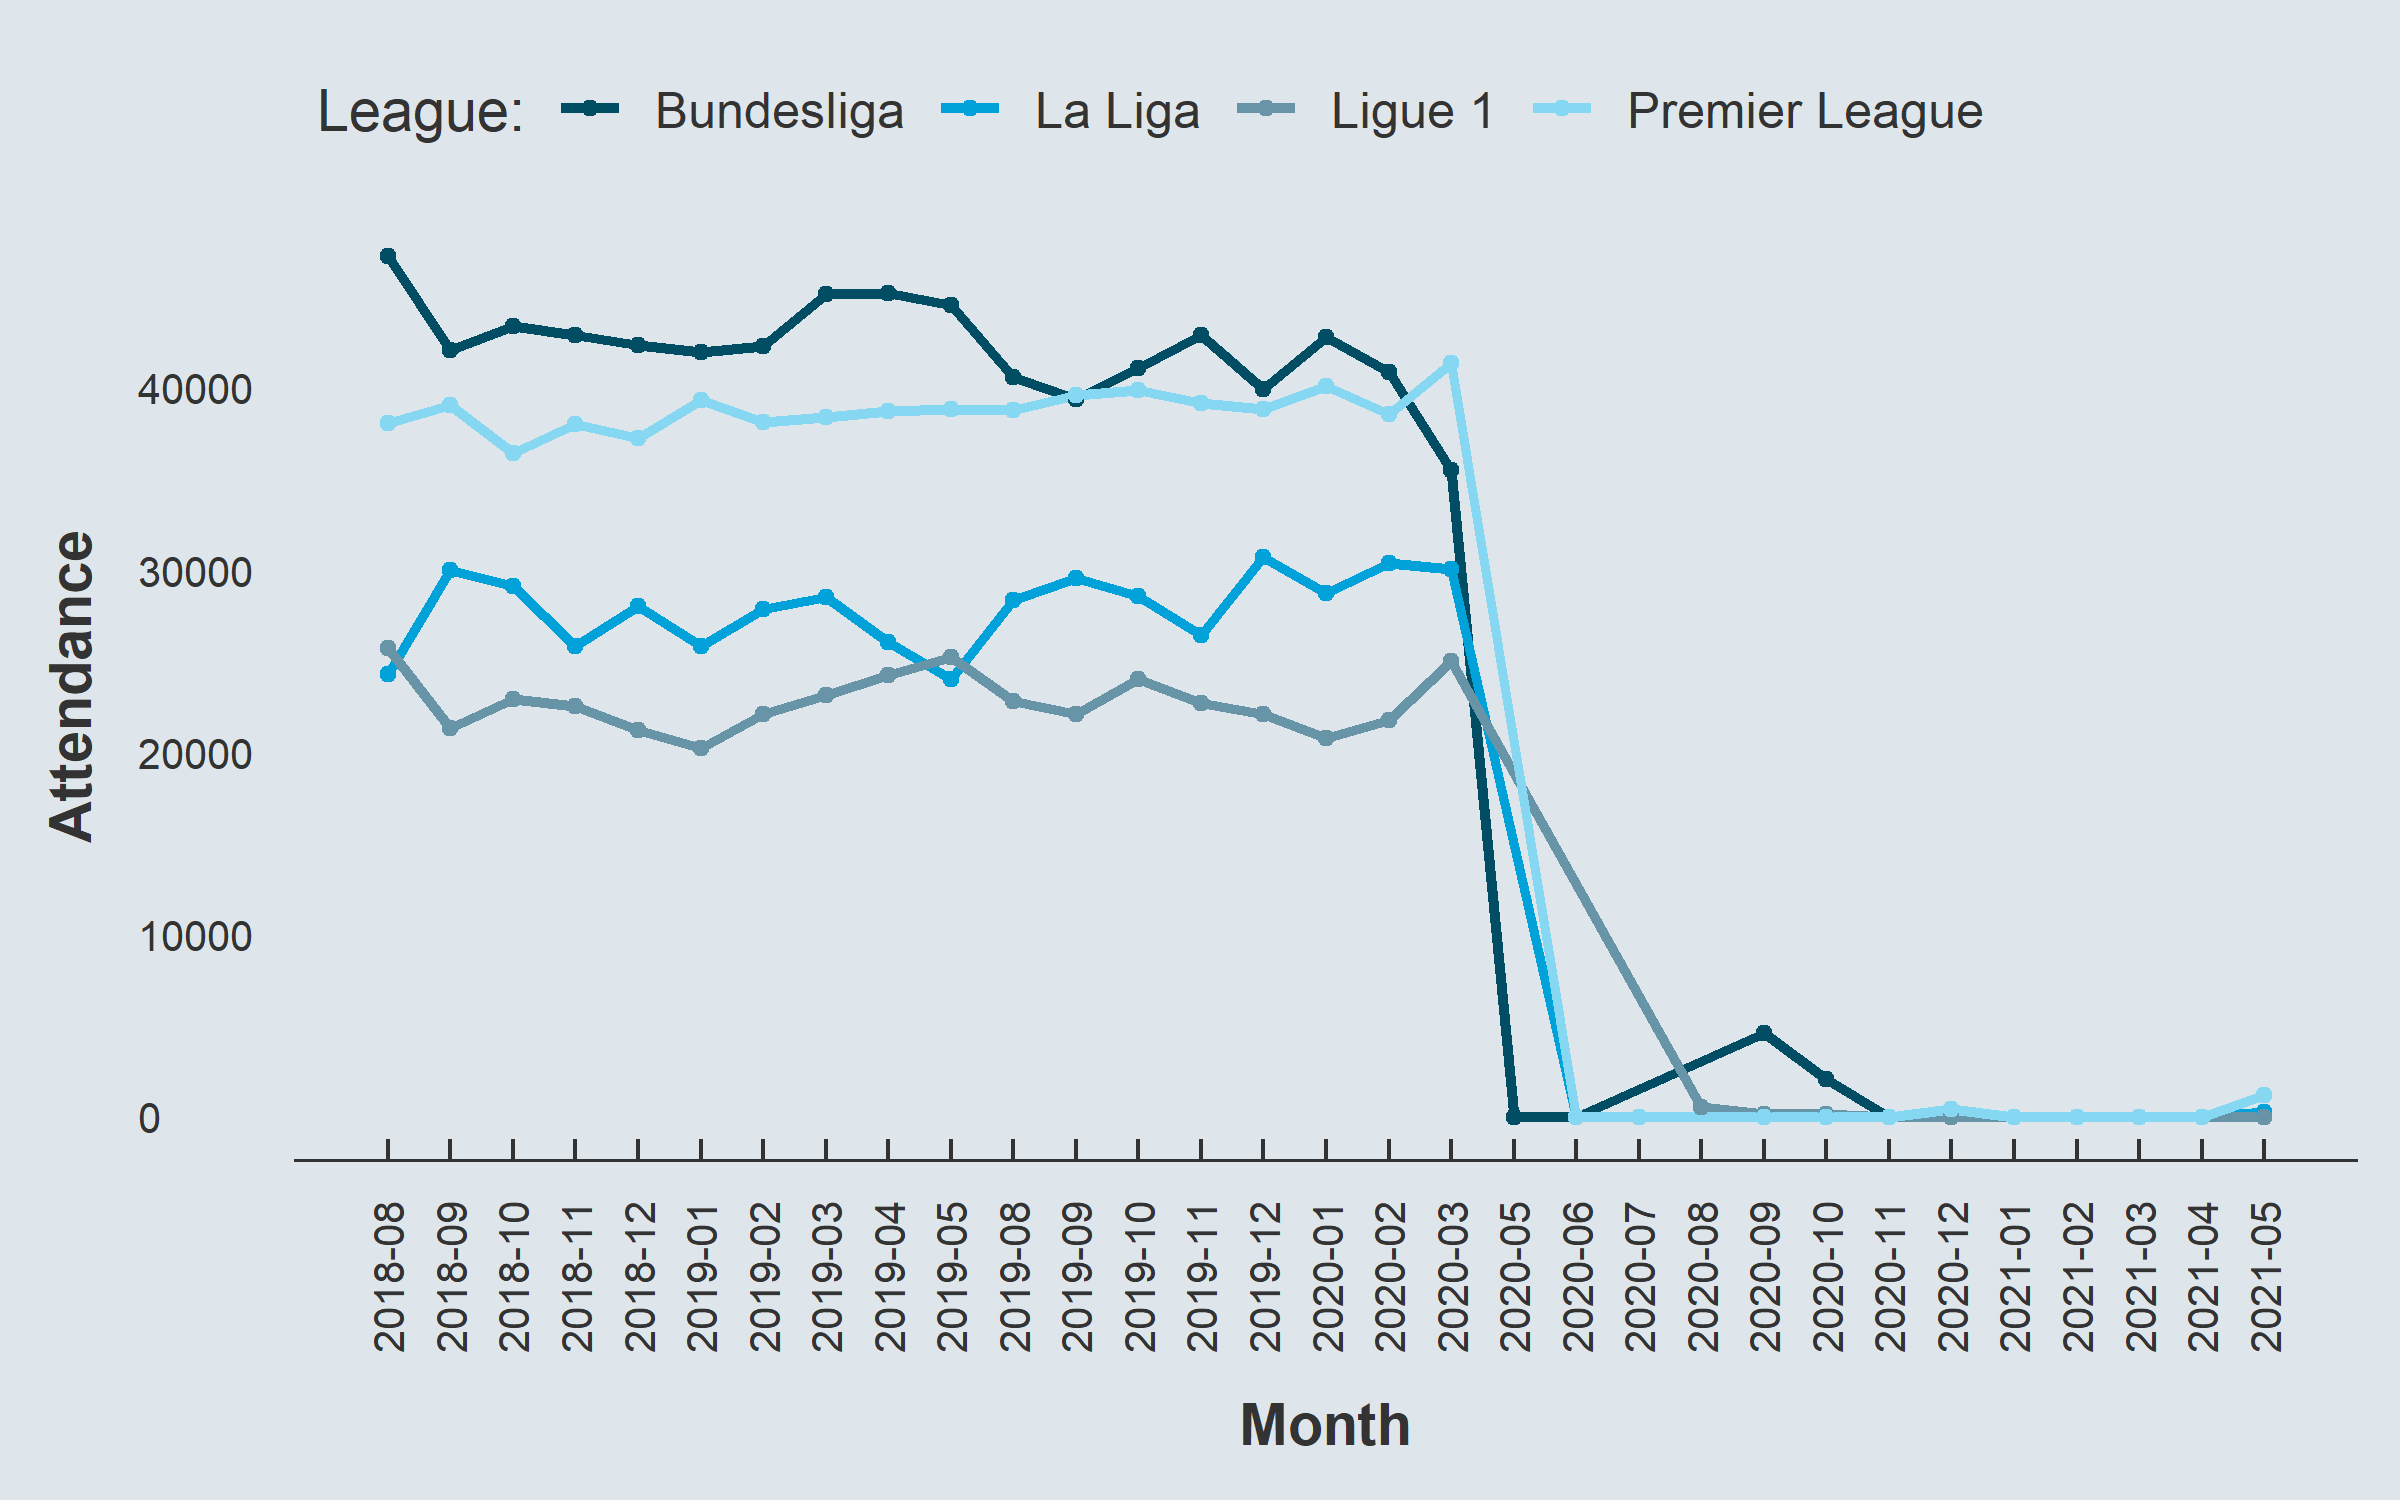
\includegraphics{example_files/figure-latex/unnamed-chunk-15-1} \end{center}

\begin{Shaded}
\begin{Highlighting}[]
\NormalTok{data_match }\OperatorTok
\StringTok{  }\CommentTok{# Put the goals scored home and away in long format}
\StringTok{  }\KeywordTok{pivot_longer}\NormalTok{(}\KeywordTok{c}\NormalTok{(Goals_home, Goals_away), }\DataTypeTok{names_to =} \StringTok{"Variable"}\NormalTok{, }\DataTypeTok{values_to =} \StringTok{"Value"}\NormalTok{) }\OperatorTok
\StringTok{  }\CommentTok{# Assign the League to the x and fill axis and the goals scored to the y axis}
\StringTok{  }\KeywordTok{ggplot}\NormalTok{(., }\KeywordTok{aes}\NormalTok{(}\DataTypeTok{x =}\NormalTok{ League, }\DataTypeTok{y =}\NormalTok{ Value, }\DataTypeTok{fill =}\NormalTok{ League)) }\OperatorTok{+}
\StringTok{  }\CommentTok{# Overlay a violin density and a boxplot with transparency}
\StringTok{  }\KeywordTok{geom_violin}\NormalTok{(}\DataTypeTok{show.legend =}\NormalTok{ F, }\DataTypeTok{alpha =} \FloatTok{.55}\NormalTok{) }\OperatorTok{+}\StringTok{ }
\StringTok{  }\KeywordTok{geom_boxplot}\NormalTok{(}\DataTypeTok{width =} \FloatTok{0.1}\NormalTok{, }\DataTypeTok{show.legend =}\NormalTok{ F, }\DataTypeTok{alpha =} \FloatTok{.75}\NormalTok{) }\OperatorTok{+}\StringTok{ }
\StringTok{  }\CommentTok{# Plot separately by season and for home/away, and custom the axes}
\StringTok{  }\KeywordTok{facet_grid}\NormalTok{(Season }\OperatorTok{~}\StringTok{ }\NormalTok{Variable) }\OperatorTok{+}\StringTok{ }\KeywordTok{ylab}\NormalTok{(}\StringTok{""}\NormalTok{) }\OperatorTok{+}\StringTok{ }\KeywordTok{xlab}\NormalTok{(}\StringTok{""}\NormalTok{) }\OperatorTok{+}
\StringTok{  }\KeywordTok{theme}\NormalTok{(}\DataTypeTok{axis.text.x =} \KeywordTok{element_text}\NormalTok{(}\DataTypeTok{angle =} \DecValTok{45}\NormalTok{, }\DataTypeTok{vjust =} \DecValTok{1}\NormalTok{, }\DataTypeTok{hjust =} \DecValTok{1}\NormalTok{)) }
\end{Highlighting}
\end{Shaded}

\begin{center}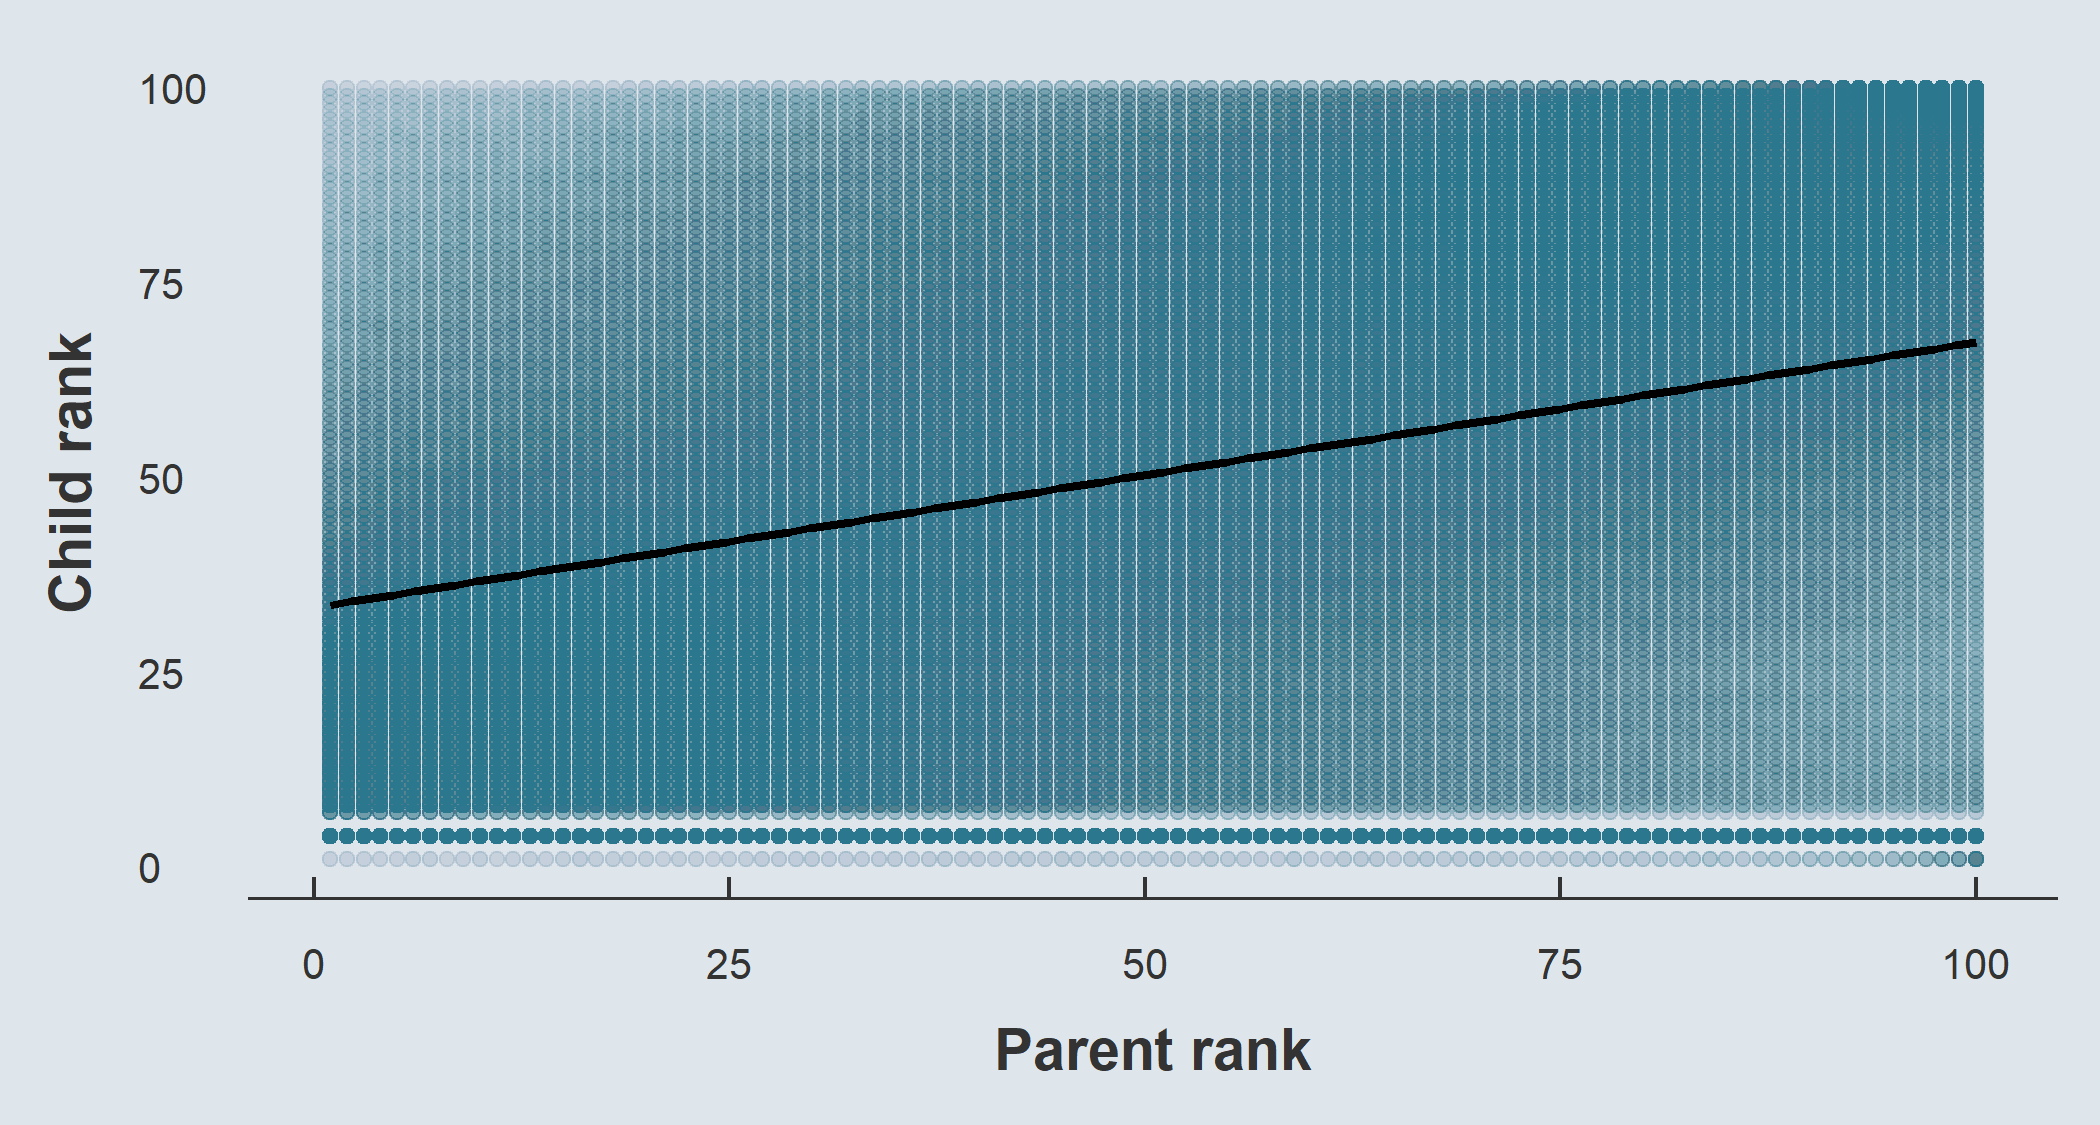
\includegraphics{example_files/figure-latex/unnamed-chunk-16-1} \end{center}

While the decline in attendance over the seasons is striking visually,
it is less the case for the difference between the distributions of the
goals scored home and those scored away. To get a more precise picture
of the evolution of the outcome of matches over the seasons, the
following graph displays the number of matches won by the home team, by
the team playing away, and the number of draws, separately for each
league and each season.

\begin{Shaded}
\begin{Highlighting}[]
\CommentTok{# Assign the League to the x axis and the outcome of the match to the fill axis}
\KeywordTok{ggplot}\NormalTok{(data_match, }\KeywordTok{aes}\NormalTok{(}\DataTypeTok{x =}\NormalTok{ League, }\DataTypeTok{fill =}\NormalTok{ Winner)) }\OperatorTok{+}
\StringTok{  }\CommentTok{# Bar plot geometry counting the number of each outcome, bars side to side}
\StringTok{  }\KeywordTok{geom_bar}\NormalTok{(}\DataTypeTok{stat =} \StringTok{"count"}\NormalTok{, }\DataTypeTok{position =} \StringTok{"dodge"}\NormalTok{, }\DataTypeTok{alpha =} \FloatTok{.85}\NormalTok{) }\OperatorTok{+}\StringTok{ }
\StringTok{  }\CommentTok{# Plot separately by season and custom the axes}
\StringTok{  }\KeywordTok{facet_wrap}\NormalTok{(}\OperatorTok{~}\NormalTok{Season) }\OperatorTok{+}\StringTok{ }\KeywordTok{ylab}\NormalTok{(}\StringTok{"Number of matches"}\NormalTok{) }\OperatorTok{+}\StringTok{ }
\StringTok{  }\KeywordTok{theme}\NormalTok{(}\DataTypeTok{axis.text.x =} \KeywordTok{element_text}\NormalTok{(}\DataTypeTok{angle =} \DecValTok{45}\NormalTok{, }\DataTypeTok{vjust =} \DecValTok{1}\NormalTok{, }\DataTypeTok{hjust =} \DecValTok{1}\NormalTok{)) }
\end{Highlighting}
\end{Shaded}

\begin{center}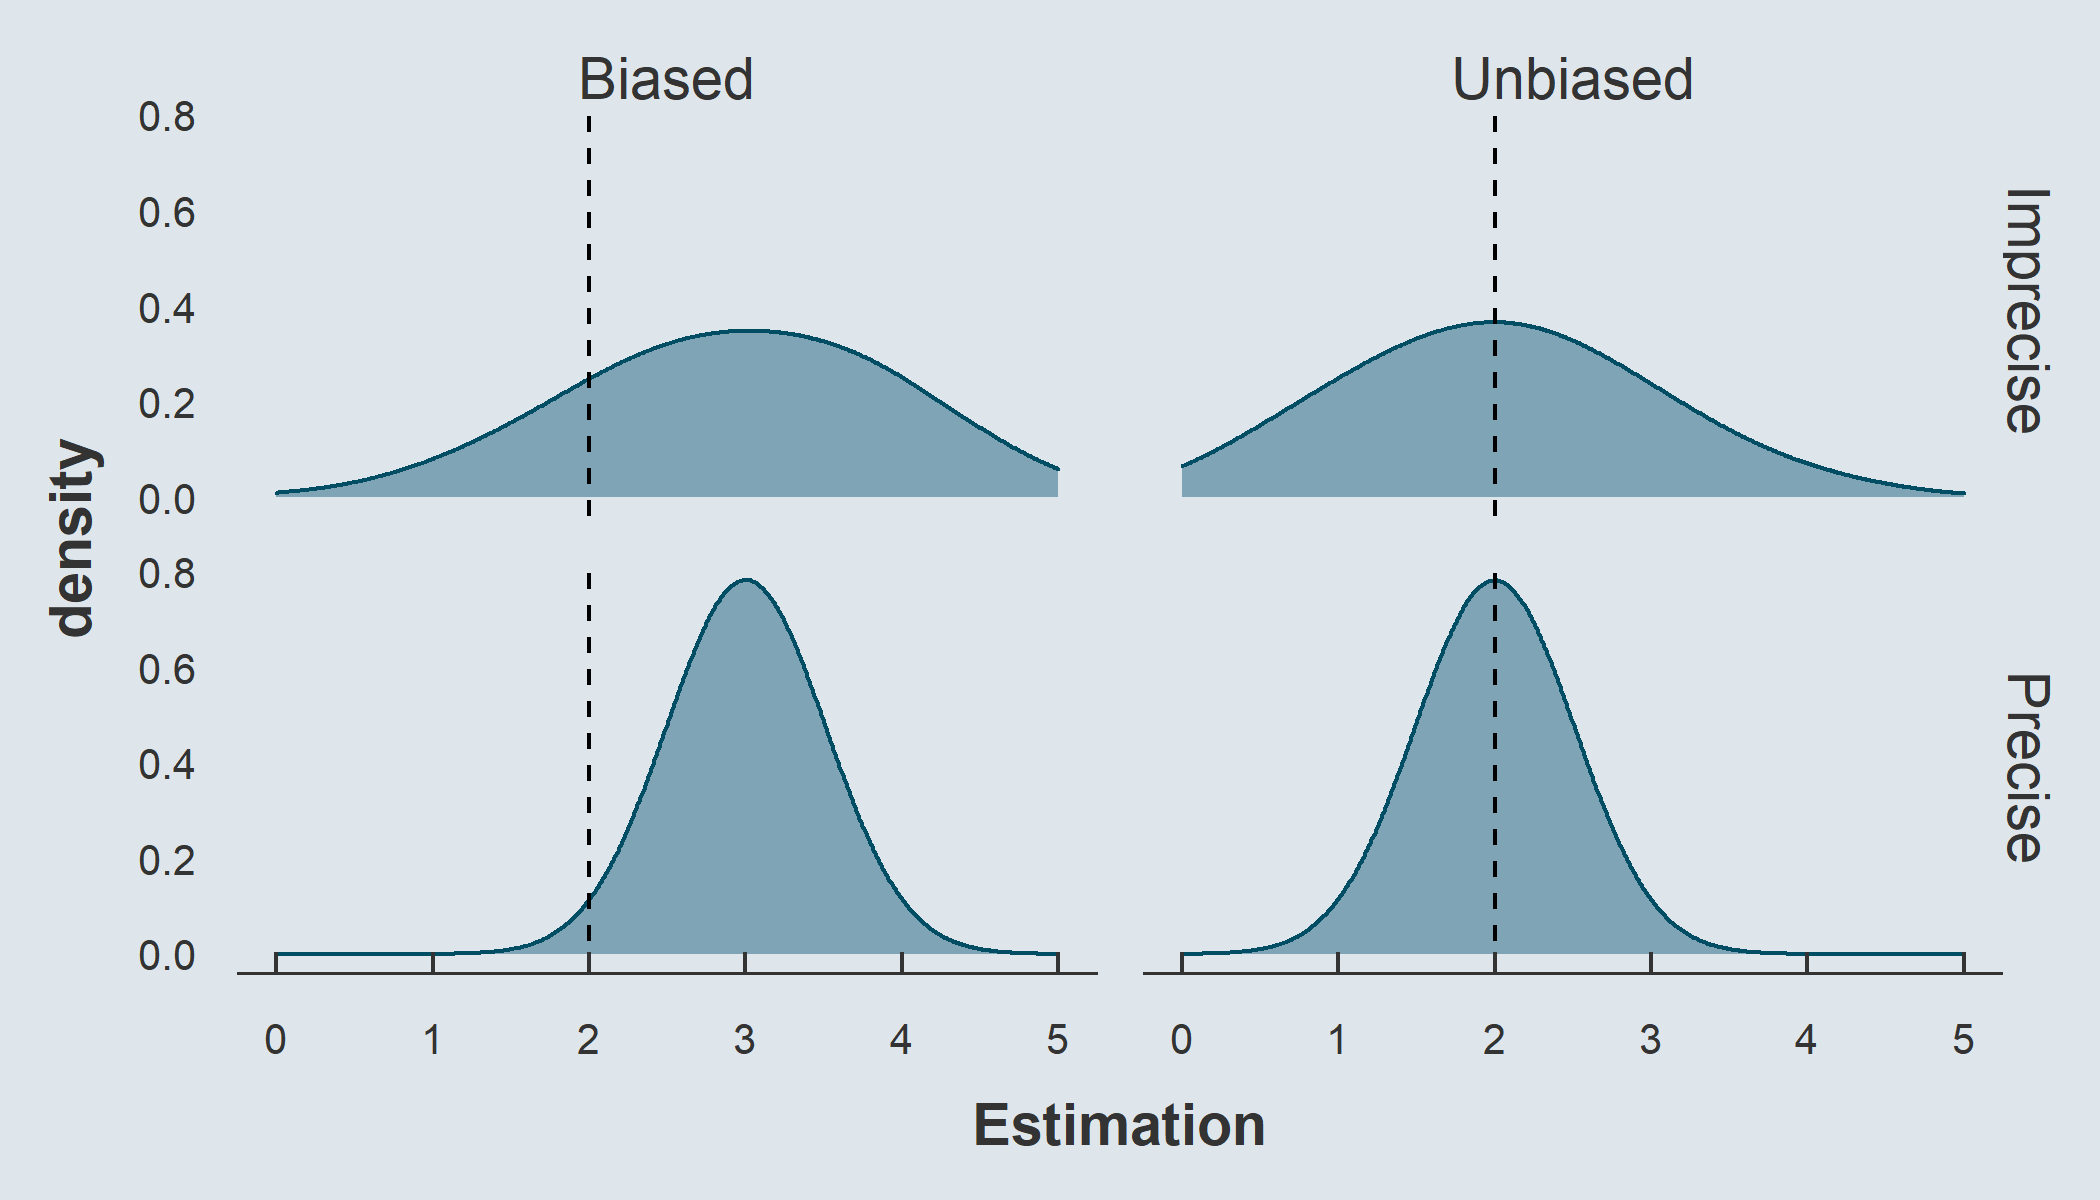
\includegraphics{example_files/figure-latex/unnamed-chunk-17-1} \end{center}

First, it confirms that the home team tends to win more frequently than
the team that plays away. But except for the Bundesliga, it is quite
clear visually that there is a decline in the difference between the
number of matches won by the team that plays home and the number of
matches won by the team that plays away, which seems concomitant with
the restrictions imposed on attendance in stadiums.

Before estimating formally the relationship between the presence of
supporters in the stadium and the probability to win the match, the
following graph compares the ratio between home wins and home losses
when there are supporters in the stadium and when there is none,
separately for each league.

\begin{Shaded}
\begin{Highlighting}[]
\CommentTok{# Generate a binary variable indicating the presence of supporters}
\NormalTok{data_match <-}\StringTok{ }\NormalTok{data_match }\OperatorTok
\StringTok{  }\KeywordTok{mutate}\NormalTok{(}\DataTypeTok{Public =} \KeywordTok{ifelse}\NormalTok{(Attendance }\OperatorTok{>}\StringTok{ }\DecValTok{0}\NormalTok{, }\StringTok{"Public"}\NormalTok{, }\StringTok{"No public"}\NormalTok{)) }

\NormalTok{data_match }\OperatorTok
\StringTok{  }\CommentTok{# Do computations separately by league and presence of supporters}
\StringTok{  }\KeywordTok{group_by}\NormalTok{(League, Public) }\OperatorTok
\StringTok{  }\CommentTok{# Compute the ratio of home vs. away wins}
\StringTok{  }\KeywordTok{summarise}\NormalTok{(}\DataTypeTok{Ratio =} \KeywordTok{sum}\NormalTok{(Winner }\OperatorTok{==}\StringTok{ "Home"}\NormalTok{) }\OperatorTok{/}\StringTok{ }\KeywordTok{sum}\NormalTok{(Winner }\OperatorTok{==}\StringTok{ "Away"}\NormalTok{)) }\OperatorTok
\StringTok{  }\CommentTok{# Assign the presence of supporters to the x axis, the ratio to the y axis,}
\StringTok{  }\CommentTok{# and the league to the color axis}
\StringTok{  }\KeywordTok{ggplot}\NormalTok{(., }\KeywordTok{aes}\NormalTok{(}\DataTypeTok{x =}\NormalTok{ Public, }\DataTypeTok{y =}\NormalTok{ Ratio, }\DataTypeTok{fill =}\NormalTok{ League), }\DataTypeTok{alpha =} \FloatTok{.85}\NormalTok{) }\OperatorTok{+}
\StringTok{  }\CommentTok{# Add a bar geometry to display the values side to side}
\StringTok{  }\KeywordTok{geom_bar}\NormalTok{(}\DataTypeTok{position =} \StringTok{"dodge"}\NormalTok{, }\DataTypeTok{stat =} \StringTok{"identity"}\NormalTok{, }\DataTypeTok{show.legend =} \OtherTok{FALSE}\NormalTok{) }\OperatorTok{+}\StringTok{ }
\StringTok{  }\CommentTok{# Plot separately for each league and custom the axes}
\StringTok{  }\KeywordTok{facet_wrap}\NormalTok{(}\OperatorTok{~}\NormalTok{League, }\DataTypeTok{nrow =} \StringTok{"1"}\NormalTok{) }\OperatorTok{+}\StringTok{ }\KeywordTok{ylab}\NormalTok{(}\StringTok{"Home wins/Home losses ratio"}\NormalTok{) }\OperatorTok{+}\StringTok{ }\KeywordTok{xlab}\NormalTok{(}\StringTok{""}\NormalTok{)}
\end{Highlighting}
\end{Shaded}

\begin{center}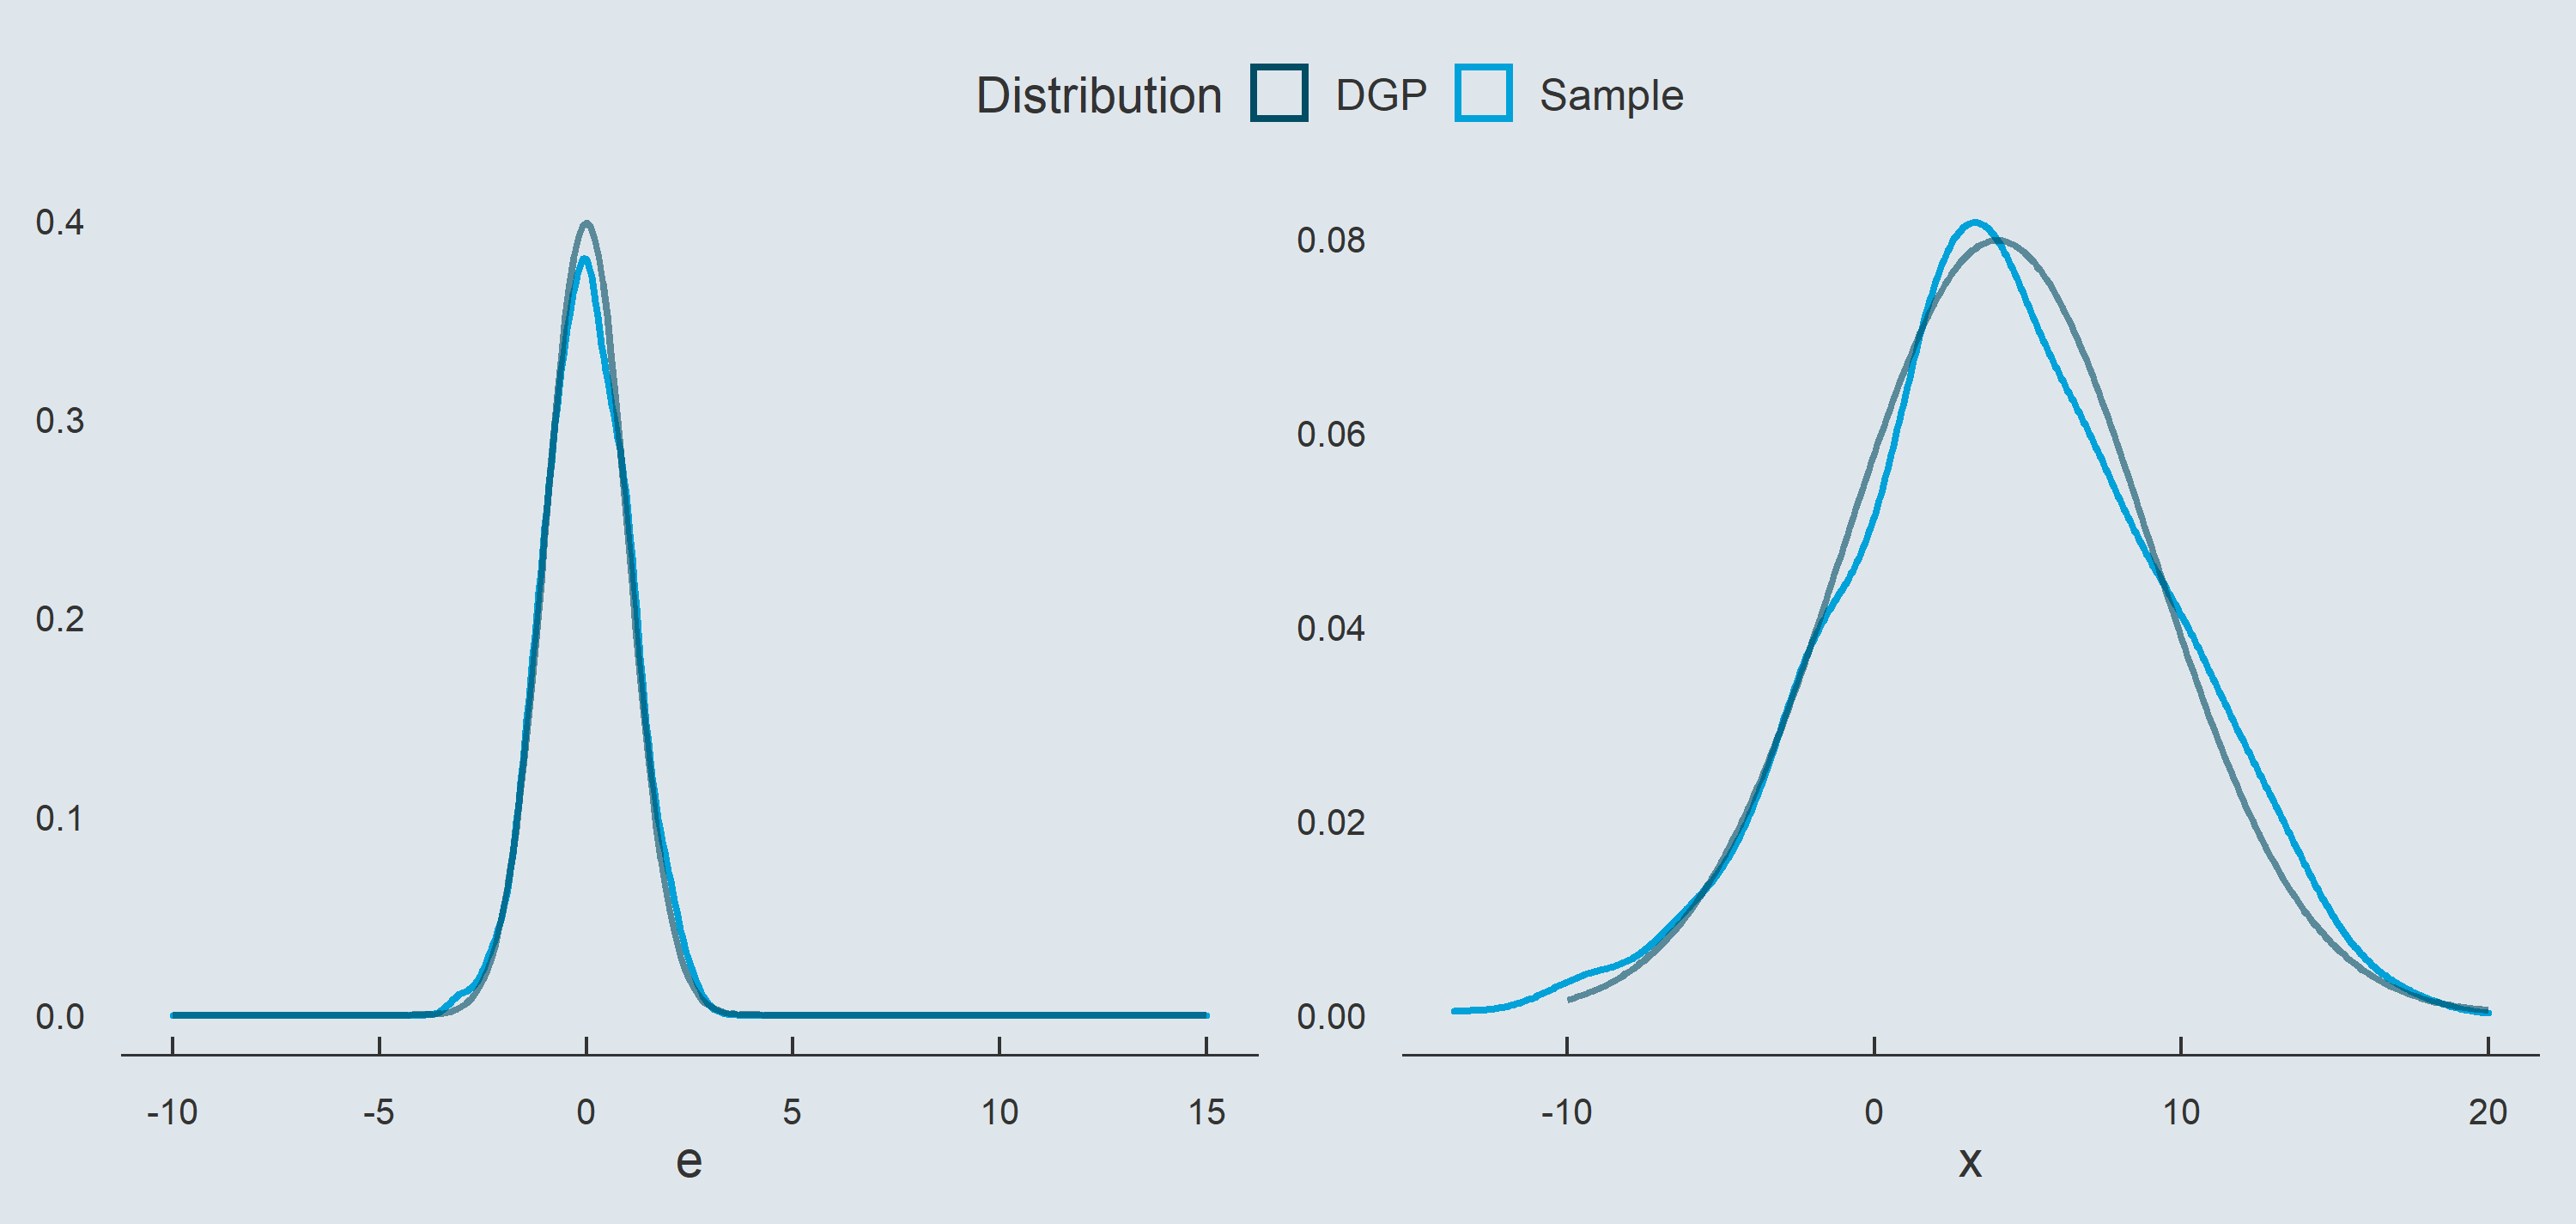
\includegraphics{example_files/figure-latex/unnamed-chunk-18-1} \end{center}

From this graph it is clear that the ratio between home wins and home
losses tends to be higher when there are supporters in the stadium than
when there is none, and that holds for the four leagues considered. But
to be able to draw clear conclusions on the relationship between the
presence of supporters in the stadium and the probability for the home
team to win the match, a regression analysis should be carried out.

\hypertarget{v.-regression-analysis}{%
\subsubsection{V. Regression analysis}\label{v.-regression-analysis}}

The equation to estimate writes:

\[1\{Winner_m=\text{Home}\}=\alpha+\beta \times1\{Public_m=\text{Yes}\}+\varepsilon_m,\]
where for a given match \(m\) the variable \(1\{Winner_m=\text{Home}\}\)
takes the value \(1\) if the winning team is that playing home and \(0\)
otherwise, and the variable \(1\{Public_m=\text{Yes}\}\) takes the value
\(1\) if there is public in the stadium and and \(0\) otherwise. Because
the dependent variable is binary, this equation corresponds to a linear
probability model and coefficients have to be interpreted in percentage
points of the probability that the home team wins the match. Because the
independent variable is binary, the constant \(\alpha\) in this model
corresponds to the probability that the home team wins the match when
there is no public, and the slope \(\beta\) corresponds to the expected
percentage-point change in this probability when there are supporters in
the stadium.

\begin{Shaded}
\begin{Highlighting}[]
\CommentTok{# Generate a binary variable that takes the value one if home team won}
\NormalTok{data_match <-}\StringTok{ }\NormalTok{data_match }\OperatorTok
\StringTok{  }\KeywordTok{mutate}\NormalTok{(}\DataTypeTok{Winner_home =} \KeywordTok{ifelse}\NormalTok{(Winner }\OperatorTok{==}\StringTok{ "Home"}\NormalTok{, }\DecValTok{1}\NormalTok{, }\DecValTok{0}\NormalTok{)) }

\CommentTok{# Estimate the regression model}
\KeywordTok{stargazer}\NormalTok{(}\KeywordTok{lm}\NormalTok{(Winner_home }\OperatorTok{~}\StringTok{ }\NormalTok{Public, data_match), }\DataTypeTok{dep.var.labels =} \KeywordTok{c}\NormalTok{(}\StringTok{"Home win"}\NormalTok{))}
\end{Highlighting}
\end{Shaded}

Dependent variable:

Home win

PublicPublic

0.059***

(0.016)

Constant

0.395***

(0.012)

Observations

4,237

Adjusted R2

0.003

Note:

⋆p\textless0.1;⋆⋆p\textless0.05;⋆⋆⋆p\textless0.01

According to these results, the presence of supporters in the audience
increases by 5.9 percentage points on expectation the probability for
the home team to win the match, everything else equal. Given that the
probability for the home team to win the match (relative to loose or
draw) is equal to 39.5\% when there is no public, this corresponds to an
average increase of about 15\% in relative terms. Given that the
p-values associated with \(\hat{\alpha}\) and \(\hat{\beta}\) are lower
than 1\%, these two values are statistically significantly different
from 0 at the 99\% confidence level.

The following plot represents the regression line estimated in the
previous table. Because both the dependent and the independent variables
are binary, each point can only take 4 locations on the graph. To
facilitate visualization, I use \texttt{geom\_jitter()} to introduce
some noise in the location of each data point around these 4 possible
coordinates. It appears that the number of home wins relative to the
number of home losses and draws is indeed lower when there is no
supporter in the stadium.

\begin{Shaded}
\begin{Highlighting}[]
\CommentTok{# Assign the dependent and the independent variables to x and y axes}
\KeywordTok{ggplot}\NormalTok{(data_match, }\KeywordTok{aes}\NormalTok{(}\DataTypeTok{x =}\NormalTok{ Public, }\DataTypeTok{y =}\NormalTok{ Winner_home)) }\OperatorTok{+}
\StringTok{  }\CommentTok{# Plot the data points with some noise to avoid overplotting}
\StringTok{  }\KeywordTok{geom_jitter}\NormalTok{(}\DataTypeTok{width =} \FloatTok{.25}\NormalTok{, }\DataTypeTok{height =} \FloatTok{.25}\NormalTok{, }\DataTypeTok{alpha =} \FloatTok{.5}\NormalTok{, }\DataTypeTok{color =} \StringTok{"#6794A7"}\NormalTok{) }\OperatorTok{+}
\StringTok{  }\CommentTok{# Plot the regression line centered with respect to the data points}
\StringTok{  }\KeywordTok{geom_smooth}\NormalTok{(}\DataTypeTok{data =}\NormalTok{ data_match }\OperatorTok\StringTok{ }
\StringTok{                }\KeywordTok{mutate}\NormalTok{(}\DataTypeTok{Public =} \KeywordTok{ifelse}\NormalTok{(Public }\OperatorTok{==}\StringTok{ "Public"}\NormalTok{, }\DecValTok{1}\NormalTok{, }\DecValTok{0}\NormalTok{) }\OperatorTok{+}\StringTok{ }\DecValTok{1}\NormalTok{), }
              \KeywordTok{aes}\NormalTok{(}\DataTypeTok{x =}\NormalTok{ Public, }\DataTypeTok{y =}\NormalTok{ Winner_home), }
              \DataTypeTok{method =} \StringTok{"lm"}\NormalTok{, }\DataTypeTok{se =}\NormalTok{ F, }\DataTypeTok{color =} \StringTok{"#014D64"}\NormalTok{) }\OperatorTok{+}
\StringTok{  }\CommentTok{# Custom the axes}
\StringTok{  }\KeywordTok{scale_x_discrete}\NormalTok{(}\DataTypeTok{name =} \StringTok{"1\{Public[m] = Yes\}"}\NormalTok{, }\DataTypeTok{labels =} \DecValTok{0}\OperatorTok{:}\DecValTok{1}\NormalTok{) }\OperatorTok{+}
\StringTok{  }\KeywordTok{ylab}\NormalTok{(}\StringTok{"Probability of winning vs. loosing home"}\NormalTok{) }
\end{Highlighting}
\end{Shaded}

\begin{center}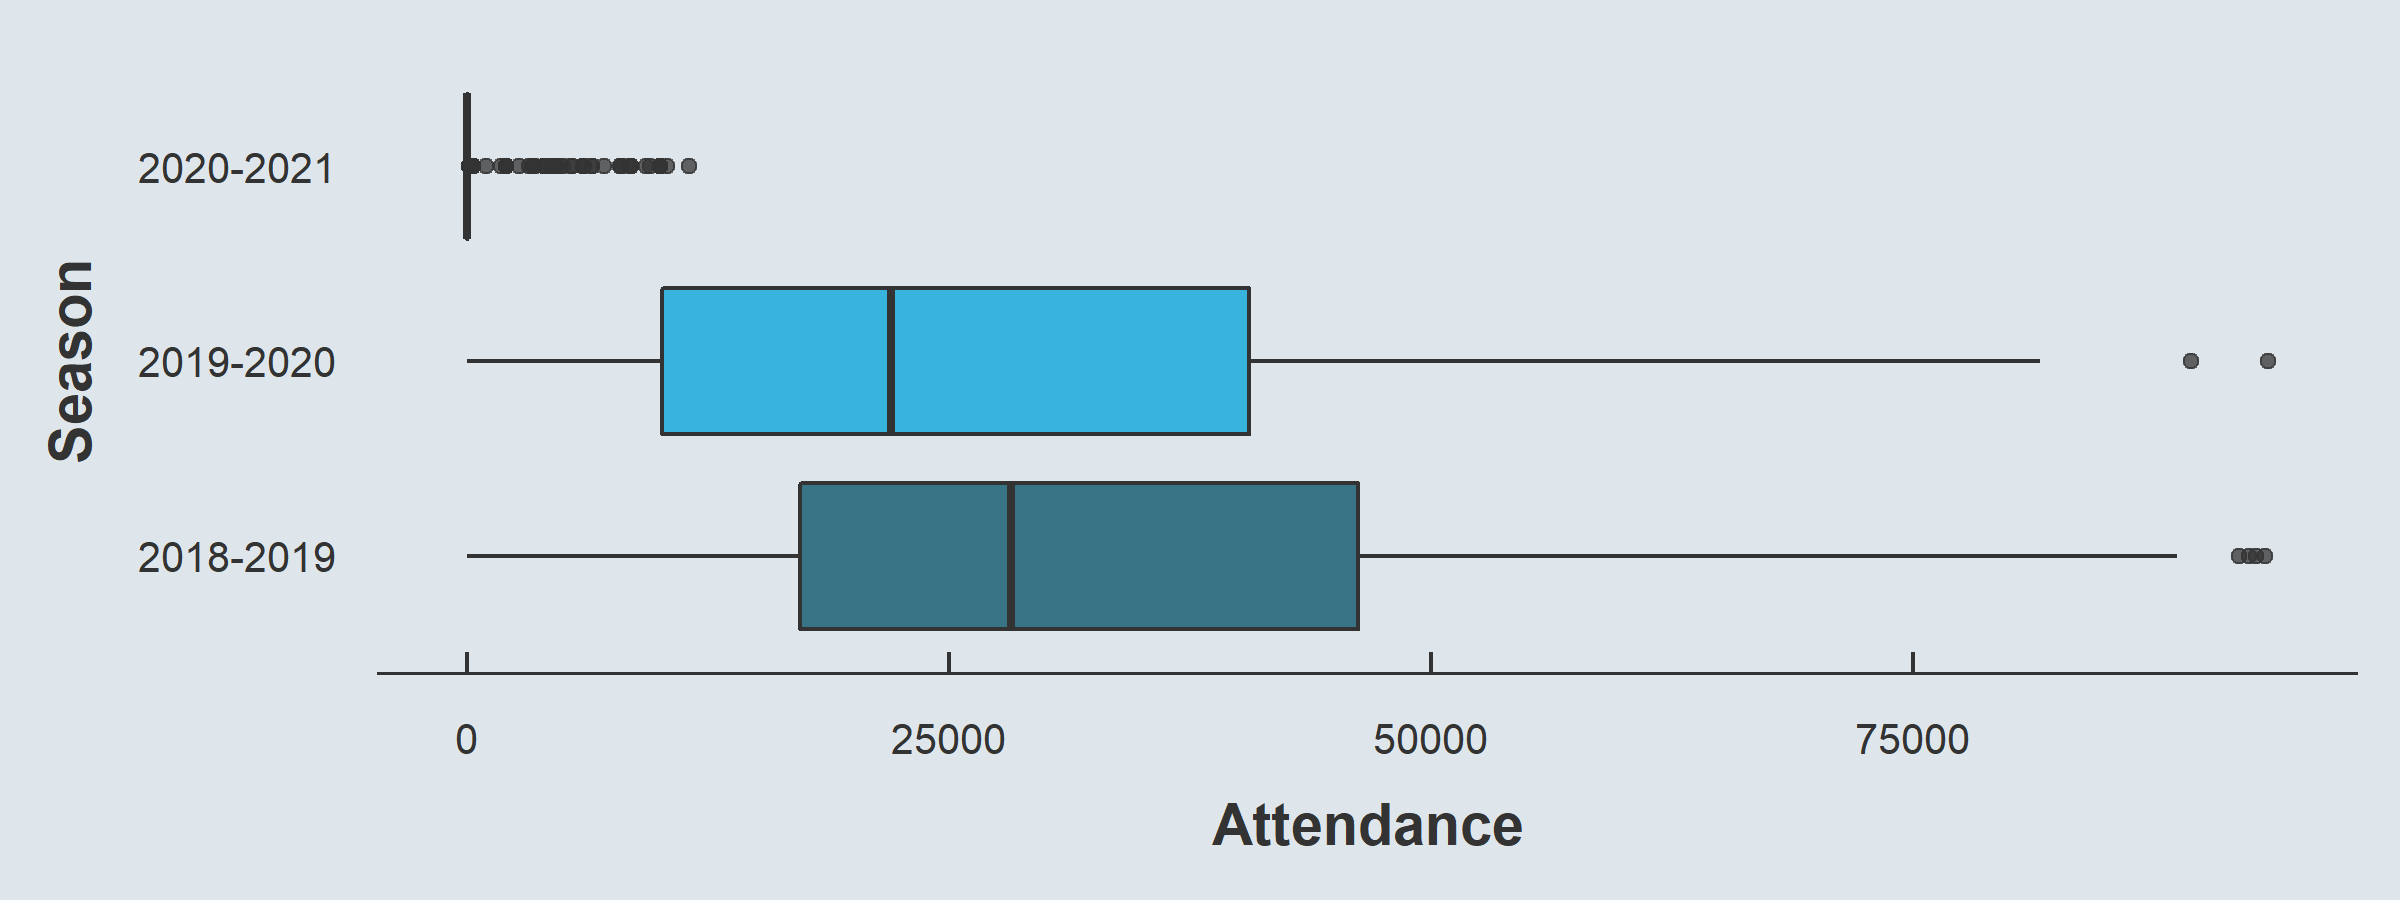
\includegraphics{example_files/figure-latex/unnamed-chunk-20-1} \end{center}

\hypertarget{vi.-causality-assessment}{%
\subsubsection{VI. Causality
assessment}\label{vi.-causality-assessment}}

The previous regression table documented a positive and statistically
significant relationship between the presence of supporters in the
stadium and the probability for the home team to win. These results
suggest the supporters have an influence on the outcome of the match, be
it directly, e.g., by impacting on the motivation of players, or
indirectly, e.g., by impacting the decisions of the referees in favor of
the home team.

But even though this result provides support for this hypothesis, it is
not sufficient to prove the presence of a causal effect. Indeed, there
may be other variables, correlated both with the dependent and the
independent variable, that drive this relationship. The COVID-19
pandemic may have simultaneously prevented supporters from going to the
stadium and changed the conditions for the team that plays away in a
favorable way, for instance if the trip to the stadium is less tiring
because there is less congestion on the roads due to remote working, or
for any other reason. In other words, there may be an omitted variable
bias driving part or all of the estimated relationship. Because it is
not feasible to control for such variables in the regression, more
sophisticated econometric specifications would be required to conclude
on the causality of the effect.

\hypertarget{vii.-robustness}{%
\subsubsection{VII. Robustness}\label{vii.-robustness}}

But even if it is not possible to include all the relevant controls,
some variables can still be added to the regression to check the
robustness of the baseline result. Indeed, if the probability
differential with and without supporters can be linked to changes in
transport conditions with the pandemic, it could also be linked to the
day in the week and the time in the day at which the match takes place,
as transport conditions may also depend on that. Thus, even though
controlling for these variables would not prove any irrelevance of the
mechanisms mentioned in the above section, it is important to check that
the baseline result is robust to the inclusion of the variables that can
be controlled for given the data available. The following table
progressively includes the league, the day of the week, and the time of
the day as controls in the regression. Because the \texttt{League}
variables is categorical, I first set a reference category to this
variable using the \texttt{relevel()} function.

\begin{Shaded}
\begin{Highlighting}[]
\CommentTok{# Set the League variable as factor and its reference category to "Premier League"}
\NormalTok{data_match <-}\StringTok{ }\NormalTok{data_match }\OperatorTok\StringTok{ }
\StringTok{  }\KeywordTok{mutate}\NormalTok{(}\DataTypeTok{League =} \KeywordTok{relevel}\NormalTok{(}\KeywordTok{as.factor}\NormalTok{(League), }\StringTok{"Premier League"}\NormalTok{))}

\CommentTok{# Progressively include control variables in the regression}
\KeywordTok{stargazer}\NormalTok{(}\KeywordTok{lm}\NormalTok{(Winner_home }\OperatorTok{~}\StringTok{ }\NormalTok{Public, data_match), }
          \KeywordTok{lm}\NormalTok{(Winner_home }\OperatorTok{~}\StringTok{ }\NormalTok{Public }\OperatorTok{+}\StringTok{ }\NormalTok{League, data_match), }
          \KeywordTok{lm}\NormalTok{(Winner_home }\OperatorTok{~}\StringTok{ }\NormalTok{Public }\OperatorTok{+}\StringTok{ }\NormalTok{League }\OperatorTok{+}\StringTok{ }\NormalTok{Day, data_match), }
          \KeywordTok{lm}\NormalTok{(Winner_home }\OperatorTok{~}\StringTok{ }\NormalTok{Public }\OperatorTok{+}\StringTok{ }\NormalTok{League }\OperatorTok{+}\StringTok{ }\NormalTok{Day }\OperatorTok{+}\StringTok{ }\NormalTok{Time, data_match),}
          \DataTypeTok{dep.var.labels =} \KeywordTok{c}\NormalTok{(}\StringTok{"Home win vs. Home loss"}\NormalTok{, }\StringTok{"Home win vs. Home loss/Draw"}\NormalTok{))}
\end{Highlighting}
\end{Shaded}

Dependent variable:

Home win vs.~Home loss

(1)

(2)

(3)

(4)

PublicPublic

0.059***

0.060***

0.060***

0.060***

(0.016)

(0.016)

(0.016)

(0.016)

LeagueBundesliga

-0.012

-0.012

-0.015

(0.022)

(0.022)

(0.022)

LeagueLa Liga

0.004

0.007

-0.001

(0.021)

(0.021)

(0.022)

LeagueLigue 1

-0.014

-0.013

-0.023

(0.021)

(0.022)

(0.023)

DayMon

-0.039

-0.040

(0.050)

(0.050)

DaySat

0.005

0.019

(0.031)

(0.033)

DaySun

-0.008

0.008

(0.031)

(0.035)

DayThu

0.006

0.009

(0.059)

(0.059)

DayTue

0.055

0.057

(0.047)

(0.047)

DayWed

0.023

0.026

(0.039)

(0.039)

Time

0.004

(0.004)

Constant

0.395***

0.400***

0.396***

0.317***

(0.012)

(0.017)

(0.034)

(0.078)

Observations

4,237

4,237

4,237

4,237

Adjusted R2

0.003

0.003

0.002

0.002

Note:

⋆p\textless0.1;⋆⋆p\textless0.05;⋆⋆⋆p\textless0.01

The baseline coefficient remains virtually unchanged in terms of
magnitude with the inclusion of control variables, and is always
statistically significantly different from 0 at 99\% confidence level.
Thus, the baseline estimate is robust to the inclusion of these three
control variables.

Another robustness check could be performed regarding the definition of
the dependent variable. Indeed, the regressions estimated so far are
about the probability of winning relative to loosing or draw. An
alternative definition would be to consider the probability of winning
relative to loosing only, omitting draws. The following table compares
the results from the baseline regression using these two possible
definitions of the independent variable.

\begin{Shaded}
\begin{Highlighting}[]
\CommentTok{# Generate an outcome variable that does not account for draws}
\NormalTok{data_match <-}\StringTok{ }\NormalTok{data_match }\OperatorTok
\StringTok{  }\KeywordTok{mutate}\NormalTok{(}\DataTypeTok{Winner_home2 =} \KeywordTok{ifelse}\NormalTok{(Winner }\OperatorTok{!=}\StringTok{ "Draw"}\NormalTok{, Winner_home, }\OtherTok{NA}\NormalTok{))}

\CommentTok{# Regress whether the home team won on the presence of supporters for these }
\CommentTok{# two definitions of the reference group}
\KeywordTok{stargazer}\NormalTok{(}\KeywordTok{lm}\NormalTok{(Winner_home }\OperatorTok{~}\StringTok{ }\NormalTok{Public, data_match), }
          \KeywordTok{lm}\NormalTok{(Winner_home2 }\OperatorTok{~}\StringTok{ }\NormalTok{Public, data_match), }
          \DataTypeTok{dep.var.labels =} \KeywordTok{c}\NormalTok{(}\StringTok{"Home win vs. Home loss"}\NormalTok{, }\StringTok{"Home win vs. Home loss/Draw"}\NormalTok{))}
\end{Highlighting}
\end{Shaded}

Dependent variable:

Home win vs.~Home loss

Home win vs.~Home loss/Draw

(1)

(2)

PublicPublic

0.059***

0.078***

(0.016)

(0.018)

Constant

0.395***

0.529***

(0.012)

(0.014)

Observations

4,237

3,170

Adjusted R2

0.003

0.006

Note:

⋆p\textless0.1;⋆⋆p\textless0.05;⋆⋆⋆p\textless0.01

Using this alternative definition, it appears that even though the
presence of supporters is associated with a higher probability to win
for the home team, even with no public the home team is still more
likely to win than the team playing away, by about 3 percentage points
(\(\hat{\alpha}>50\%\)). The coefficient of interest is statistically
significantly different from 0 at 99\% confidence level for both
variable definitions. In terms of magnitude, the coefficients from the
two definitions cannot be compared directly because they are
mechanically inflated by the omission of the possibility of draw, but
the ratio of the effect of public in the stadium on the probability to
win, relative to the probability to win when there is no public, is very
similar in the two cases
(\(\frac{0.059}{0.395}\)\(=\)\(0.1494\)\(\approx\)\(0.1475\)\(=\)\(\frac{0.078}{0.529}\)).
It is thus reasonable to conclude that this result is also robust to
variations in the definition of the reference category of the outcome
variable.

\hypertarget{viii.-heterogeneity}{%
\subsubsection{VIII. Heterogeneity}\label{viii.-heterogeneity}}

But the fact that the coefficient is robust does not mean that it is
homogeneous. To investigate whether the relationship differs from one
league to another, the independent variable of interest should be
interacted with the \texttt{League} variable, which is equivalent to
estimating the regression separately for each league.

\begin{Shaded}
\begin{Highlighting}[]
\CommentTok{# Progressively control and interact with League in the regression}
\KeywordTok{stargazer}\NormalTok{(}\KeywordTok{lm}\NormalTok{(Winner_home }\OperatorTok{~}\StringTok{ }\NormalTok{Public, data_match),}
          \KeywordTok{lm}\NormalTok{(Winner_home }\OperatorTok{~}\StringTok{ }\NormalTok{Public }\OperatorTok{+}\StringTok{ }\NormalTok{League, data_match),}
          \KeywordTok{lm}\NormalTok{(Winner_home }\OperatorTok{~}\StringTok{ }\NormalTok{Public }\OperatorTok{+}\StringTok{ }\NormalTok{League }\OperatorTok{+}\StringTok{ }\NormalTok{Public }\OperatorTok{*}\StringTok{ }\NormalTok{League, data_match),}
          \DataTypeTok{dep.var.labels =} \KeywordTok{c}\NormalTok{(}\StringTok{"Home win"}\NormalTok{))}
\end{Highlighting}
\end{Shaded}

Dependent variable:

Home win

(1)

(2)

(3)

PublicPublic

0.059***

0.060***

0.074**

(0.016)

(0.016)

(0.030)

LeagueBundesliga

-0.012

0.008

(0.022)

(0.035)

LeagueLa Liga

0.004

0.019

(0.021)

(0.032)

LeagueLigue 1

-0.014

-0.016

(0.021)

(0.034)

PublicPublic:LeagueBundesliga

-0.032

(0.045)

PublicPublic:LeagueLa Liga

-0.025

(0.042)

PublicPublic:LeagueLigue 1

0.002

(0.044)

Constant

0.395***

0.400***

0.392***

(0.012)

(0.017)

(0.023)

Observations

4,237

4,237

4,237

Adjusted R2

0.003

0.003

0.002

Note:

⋆p\textless0.1;⋆⋆p\textless0.05;⋆⋆⋆p\textless0.01

Column (3) shows that the coefficient of interest for the reference
category, Premier League, amounts to 7.4 percentage points and is
statistically different from 0 at the 95\% confidence level. The
difference between the effect in Premier League and that in other
leagues range from -3.2 percentage points (i.e., an effect of 4.2
percentage points, for Bundesliga) to 0.2 percentage points (i.e., an
effect of 7.6 percentage points, for Ligue 1). Yet, because the
coefficients associated with the interaction terms are not significant,
we cannot conclude that these different league-specific effects are
statistically significant from each other. In other words, there is no
evidence of a heterogeneity of the effect across leagues.

\hypertarget{ix.-conclusion}{%
\subsubsection{IX. Conclusion}\label{ix.-conclusion}}

In this analysis I use data on football matches in Premier League, Ligue
1, La Liga, and Bundesliga, from season 2018-2019 to season 2020-2021,
to investigate the relationship between the presence of supporters in
the stadium and the probability for the football team that plays home to
win the match. The estimation of this relationship relies on the fact
that the COVID-19 pandemic prevented supporters from going to the
stadium, such that the outcome of these matches can be compared to those
played in regular conditions. Graphical evidence indeed show a clear and
sudden drop to 0 attendance in stadiums, concomitant to the pandemic
right after March 2020.

Results show that the presence of supporters in the audience increases
by 5.9 percentage points on expectation the probability for the home
team to win the match, everything else equal. Yet, this result may not
be interpreted as causal if the COVID-19 pandemic have simultaneously
prevented supporters from going to the stadium and changed the
conditions for the team that plays away relative to the conditions for
the team that plays home. In addition, the external validity of the
result is not granted, as it is estimated using four European football
leagues only. Still, the estimated coefficient appears to be robust to
controlling for the league, the day of the week, and the time of the
day, as well as changes in the definition of the outcome variable, and
results show no evidence for a heterogeneity of the effect across
leagues.

\hypertarget{references}{%
\subsubsection{References}\label{references}}

Dowie, J. (1982). Why Spain should win the world cup. \emph{New
Scientist}, 94(10), 693-695.

Greer, D. L. (1983). Spectator booing and the home advantage: A study of
social influence in the basketball arena. \emph{Social psychology
quarterly}, 252-261.

Loughead, T. M., Carron, A. V., Bray, S. R., \& Kim, A. J. (2003).
Facility familiarity and the home advantage in professional sports.
\emph{International Journal of Sport and Exercise Psychology}, 1(3),
264-274.

Pollard, R. (1986). Home advantage in soccer: A retrospective analysis.
\emph{Journal of sports sciences}, 4(3), 237-248.

Pollard, R., Silva, C. D., \& Medeiros, N. C. (2008). Home advantage in
football in Brazil: differences between teams and the effects of
distance traveled. \emph{Revista Brasileira de Futebol (The Brazilian
Journal of Soccer Science)}, 1(1), 3-10.

⚽

\end{document}
